%
% This work is licensed under a Creative Commons Attribution-ShareAlike 4.0 International License.
% http://creativecommons.org/licenses/by-sa/4.0/
%
\documentclass{beamer}
\usetheme[pageofpages=of,% String used between the current page and the
                         % total page count.
          bullet=circle,% Use circles instead of squares for bullets.
          titleline=true,% Show a line below the frame title.
          alternativetitlepage=true,% Use the fancy title page.
	  titlepagelogo=images/logoM-circl-Forensics.png,% Logo for the first page.
%          watermark=watermark-polito,% Watermark used in every page.
%          watermarkheight=100px,% Height of the watermark.
%          watermarkheightmult=4,% The watermark image is 4 times bigger
                                % than watermarkheight.
          ]{Torino}

\usepackage[utf8]{inputenc}
\usepackage{listings}
\usepackage{color}
\usepackage[font=small,labelfont=bf]{caption}
\usepackage{transparent}
\usepackage{siunitx}

\usepackage[norndcorners,customcolors]{hf-tikz}
\hfsetbordercolor{yellow}
\hfsetfillcolor{yellow}

\lstset{ 
  backgroundcolor=\color{white},   % choose the background color; you must add \usepackage{color} or \usepackage{xcolor}
  basicstyle=\footnotesize,        % the size of the fonts that are used for the code
  breakatwhitespace=false,
}


\author{CIRCL \emph{TLP:CLEAR}}
\title{CIRCL - Digital Forensics 1.0.2}
\subtitle{Introduction: File System Forensics and Data Recovery}
\institute{info@circl.lu}
\date{December, 2024}



\begin{document}
\begin{frame}[t,plain]
\titlepage
\end{frame}


\begin{frame}
  \frametitle{Overview}
  \begin{itemize}
  \item[]
      \begin{enumerate}
          \item File System Analysis - Abstract
          \item FAT - File Allocation Table
          \item NTFS - New Technology File System
          \item NTFS - Advanced
          \item File System Time Line
          \item 
          \item Carving and String Search
          \item Forensics Challenges
          \item Bibliography and Outlook
      \end{enumerate}
  \end{itemize}
\end{frame}


%
% This work is licensed under a Creative Commons Attribution-ShareAlike 4.0 International License.
% http://creativecommons.org/licenses/by-sa/4.0/
%

% DO NOT COMPILE THIS FILE DIRECTLY!
% This is included by the other .tex files.


\begin{frame}
    \includegraphics[scale=0.3]{images/logo-circl-Forensics.png}
    \begin{itemize}
        \item[]
        \item[]
        \item[] 1. File System Analysis - Abstract
    \end{itemize}
\end{frame}


\begin{frame}[fragile]
  \frametitle{1.1 Organizing data in files}
  \begin{lstlisting}[basicstyle=\tiny\ttfamily]
             - Organizing data on a volume
             - Maintain file related meta data
             - Maintain allocation status of clusters
                            

                Metadata                                   Content     
    ----------------------------------       ----------------------------------
  1 |                                |       |                                | 5001
    |                                |       |                                | 5002
    |                                |       |                                | 5003
    |                                |       |                                | 5004
    |                                |       |                                | 5005
    |--------------------------------|       |                                | 5006
  2 |                                |       |                                | ...
    |                                |       |                                | ...
    |                                |       |                                | ...
    |                                |       |                                | ...
    |                                |       |                                | ...
    ----------------------------------       |                                | ...
  3 |                                |       |                                | ...
    |             .....              |       |                                | 5014
    ----------------------------------       ----------------------------------
                                              |       |       |       |      |
                                              0       8      16      24     31


       Allocation table:
  \end{lstlisting}
\end{frame}


\begin{frame}[fragile]
  \frametitle{1.1 Organizing data in files}
  \begin{lstlisting}[basicstyle=\tiny\ttfamily]
             - Organizing data on a volume
             - Maintain file related meta data
             - Maintain allocation status of clusters
                            

                Metadata                                   Content     
    ----------------------------------       ----------------------------------
  1 |                                |       |11111111111111111111111111111111| 5001
    |                                |       |11111111111111111111111111111111| 5002
    |                                |       |1111                            | 5003
    |                                |       |                                | 5004
    |                                |       |                                | 5005
    |--------------------------------|       |                                | 5006
  2 |                                |       |                                | ...
    |                                |       |                                | ...
    |                                |       |                                | ...
    |                                |       |                                | ...
    |                                |       |                                | ...
    ----------------------------------       |                                | ...
  3 |                                |       |                                | ...
    |             .....              |       |                                | 5014
    ----------------------------------       ----------------------------------
                                              |       |       |       |      |
                                              0       8      16      24     31


       Allocation table:
  \end{lstlisting}
\end{frame}


\begin{frame}[fragile]
  \frametitle{1.1 Organizing data in files}
  \begin{lstlisting}[basicstyle=\tiny\ttfamily]
             - Organizing data on a volume
             - Maintain file related meta data
             - Maintain allocation status of clusters
                            

                Metadata                                   Content     
    ----------------------------------       ----------------------------------
  1 | Filename: file01.txt           |       |11111111111111111111111111111111| 5001
    | Time stamps: MACB              |       |11111111111111111111111111111111| 5002
    | Rights: Owner, Group, All      |       |1111                            | 5003
    | Size: 68 Byte                  |       |                                | 5004
    | Clusters: 5001,5002,5003       |       |                                | 5005
    |--------------------------------|       |                                | 5006
  2 |                                |       |                                | ...
    |                                |       |                                | ...
    |                                |       |                                | ...
    |                                |       |                                | ...
    |                                |       |                                | ...
    ----------------------------------       |                                | ...
  3 |                                |       |                                | ...
    |             .....              |       |                                | 5014
    ----------------------------------       ----------------------------------
                                              |       |       |       |      |
                                              0       8      16      24     31


       Allocation table: 5001, 5002, 5003
  \end{lstlisting}
\end{frame}


\begin{frame}[fragile]
  \frametitle{1.1 Organizing data in files}
  \begin{lstlisting}[basicstyle=\tiny\ttfamily]
             - Organizing data on a volume
             - Maintain file related meta data
             - Maintain allocation status of clusters
                            

                Metadata                                   Content     
    ----------------------------------       ----------------------------------
  1 | Filename: file01.txt           |       |11111111111111111111111111111111| 5001
    | Time stamps: MACB              |       |11111111111111111111111111111111| 5002
    | Rights: Owner, Group, All      |       |1111                            | 5003
    | Size: 68 Byte                  |       |22222222222222222222222222222222| 5004
    | Clusters: 5001,5002,5003       |       |22222222222222222222222         | 5005
    |--------------------------------|       |                                | 5006
  2 | Filename: file02.txt           |       |                                | ...
    | Time stamps: MACB              |       |                                | ...
    | Rights: Owner, Group, All      |       |                                | ...
    | Size: 55 Byte                  |       |                                | ...
    | Clusters: 5004, 5005           |       |                                | ...
    ----------------------------------       |                                | ...
  3 |                                |       |                                | ...
    |             .....              |       |                                | 5014
    ----------------------------------       ----------------------------------
                                              |       |       |       |      |
                                              0       8      16      24     31


       Allocation table: 5001, 5002, 5003, 5004, 5005
  \end{lstlisting}
\end{frame}


\begin{frame}[fragile]
  \frametitle{1.2 Deleting a file}
  \begin{lstlisting}[basicstyle=\tiny\ttfamily]
             - Organizing data on a volume
             - Maintain file related meta data
             - Maintain allocation status of clusters
                            

                Metadata                                   Content     
    ----------------------------------       ----------------------------------
  1 | Filename: file01.txt           |       |11111111111111111111111111111111| 5001
    | Time stamps: MACB              |       |11111111111111111111111111111111| 5002
    | Rights: Owner, Group, All      |       |1111                            | 5003
    | Size: 68 Byte                  |       |22222222222222222222222222222222| 5004
    | Clusters: 5001,5002,5003       |       |22222222222222222222222         | 5005
    |--------------------------------|       |                                | 5006
  2 | Filename: file02.txt (deleted) |       |                                | ...
    | Time stamps: MACB              |       |                                | ...
    | Rights: Owner, Group, All      |       |                                | ...
    | Size: 55 Byte                  |       |                                | ...
    | Clusters: 5004, 5005           |       |                                | ...
    ----------------------------------       |                                | ...
  3 |                                |       |                                | ...
    |             .....              |       |                                | 5014
    ----------------------------------       ----------------------------------
                                              |       |       |       |      |
                                              0       8      16      24     31


       Allocation table: 5001, 5002, 5003
  \end{lstlisting}
\end{frame}


\begin{frame}[fragile]
  \frametitle{1.3 Slack space - FileSlack}
  \begin{lstlisting}[basicstyle=\tiny\ttfamily]
             - Metadata: Case 1: Re-Use Metadata
             - Content: End of sector: Filled with zeros (RAM slack)
	     - Content: End of cluter: Don't touch (File slack)
                            

                Metadata                                   Content     
    ----------------------------------       ----------------------------------
  1 | Filename: file01.txt           |       |11111111111111111111111111111111| 5001
    | Time stamps: MACB              |       |11111111111111111111111111111111| 5002
    | Rights: Owner, Group, All      |       |1111                            | 5003
    | Size: 68 Byte                  |       |3333333333      2222222222222222| 5004
    | Clusters: 5001,5002,5003       |       |22222222222222222222222         | 5005
    |--------------------------------|       |                                | 5006
  2 | Filename: file03.txt           |       |                                | ...
    | Time stamps: MACB              |       |                                | ...
    | Rights: Owner, Group, All      |       |                                | ...
    | Size: 10 Byte                  |       |                                | ...
    | Clusters: 5004                 |       |                                | ...
    ----------------------------------       |                                | ...
  3 |                                |       |                                | ...
    |             .....              |       |                                | 5014
    ----------------------------------       ----------------------------------
                                              |       |       |       |      |
                                              0       8      16      24     31
 

       Allocation table: 5001, 5002, 5003, 5004
  \end{lstlisting}
\end{frame}


\begin{frame}[fragile]
  \frametitle{1.3 Slack space - FileSlack}
  \begin{lstlisting}[basicstyle=\tiny\ttfamily]
             - Metadata: Case 2: New Metadata
             - Content: End of sector: Filled with zeros (RAM slack)
	     - Content: End of cluter: Don't touch (File slack)
                            

                Metadata                                   Content     
    ----------------------------------       ----------------------------------
  1 | Filename: file01.txt           |       |11111111111111111111111111111111| 5001
    | Time stamps: MACB              |       |11111111111111111111111111111111| 5002
    | Rights: Owner, Group, All      |       |1111                            | 5003
    | Size: 68 Byte                  |       |3333333333      2222222222222222| 5004
    | Clusters: 5001,5002,5003       |       |22222222222222222222222         | 5005
    |--------------------------------|       |                                | 5006
  2 | Filename: file02.txt (deleted) |       |                                | ...
    | Time stamps: MACB              |       |                                | ...
    | Rights: Owner, Group, All      |       |                                | ...
    | Size: 55 Byte                  |       |                                | ...
    | Clusters: 5004, 5005           |       |                                | ...
    ----------------------------------       |                                | ...
  3 | Filename: file03.txt           |       |                                | ...
    | Time stamps: MACB              |       |                                | 5014
    | Rights: Owner, Group, All      |       ----------------------------------
    | Size: 10 Byte                  |        |       |       |       |      |
    | Clusters: 5004                 |        0       8      16      24     31
    ----------------------------------

       Allocation table: 5001, 5002, 5003, 5004
  \end{lstlisting}
\end{frame}


\begin{frame}[fragile]
  \frametitle{1.4 Data Recovery}
  \begin{lstlisting}[basicstyle=\tiny\ttfamily]
               # Recover sectors
               # Read from disk and write into a file
	       dd if=deleted.raw of=file02.txt bs=32 skip=5003 count=2
                            

                Metadata                                   Content     
    ----------------------------------       ----------------------------------
  1 | Filename: file01.txt           |       |11111111111111111111111111111111| 5001
    | Time stamps: MACB              |       |11111111111111111111111111111111| 5002
    | Rights: Owner, Group, All      |       |1111                            | 5003
    | Size: 68 Byte                  |       |3333333333      2222222222222222| 5004
    | Clusters: 5001,5002,5003       |       |22222222222222222222222         | 5005
    |--------------------------------|       |                                | 5006
  2 | Filename: file02.txt (deleted) |       |                                | ...
    | Time stamps: MACB              |       |                                | ...
    | Rights: Owner, Group, All      |       |                                | ...
    | Size: 55 Byte                  |       |                                | ...
    | Clusters: 5004, 5005           |       |                                | ...
    ----------------------------------       |                                | ...
  3 | Filename: file03.txt           |       |                                | ...
    | Time stamps: MACB              |       |                                | 5014
    | Rights: Owner, Group, All      |       ----------------------------------
    | Size: 10 Byte                  |        |       |       |       |      |
    | Clusters: 5004                 |        0       8      16      24     31
    ----------------------------------

       Allocation table: 5001, 5002, 5003, 5004
  \end{lstlisting}
\end{frame}


\begin{frame}[fragile]
  \frametitle{1.4 Data Recovery}
  \begin{lstlisting}[basicstyle=\tiny\ttfamily]
	       # Recover exisiting (deleted) file
               # Based on metadata
	       icat deleted.raw 3 > file03.txt
                            

                Metadata                                   Content     
    ----------------------------------       ----------------------------------
  1 | Filename: file01.txt           |       |11111111111111111111111111111111| 5001
    | Time stamps: MACB              |       |11111111111111111111111111111111| 5002
    | Rights: Owner, Group, All      |       |1111                            | 5003
    | Size: 68 Byte                  |       |3333333333      2222222222222222| 5004
    | Clusters: 5001,5002,5003       |       |22222222222222222222222         | 5005
    |--------------------------------|       |                                | 5006
  2 | Filename: file02.txt (deleted) |       |                                | ...
    | Time stamps: MACB              |       |                                | ...
    | Rights: Owner, Group, All      |       |                                | ...
    | Size: 55 Byte                  |       |                                | ...
    | Clusters: 5004, 5005           |       |                                | ...
    ----------------------------------       |                                | ...
  3 | Filename: file03.txt (deleted) |       |                                | ...
    | Time stamps: MACB              |       |                                | 5014
    | Rights: Owner, Group, All      |       ----------------------------------
    | Size: 10 Byte                  |        |       |       |       |      |
    | Clusters: 5004                 |        0       8      16      24     31
    ----------------------------------

       Allocation table: 5001, 5002, 5003
  \end{lstlisting}
\end{frame}


\begin{frame}[fragile]
  \frametitle{1.4 Data Recovery}
  \begin{lstlisting}[basicstyle=\tiny\ttfamily]
	       # Recover overwritten file
               # Based on metadata
	       icat deleted.raw 2 > file02.txt
                            

                Metadata                                   Content     
    ----------------------------------       ----------------------------------
  1 | Filename: file01.txt           |       |11111111111111111111111111111111| 5001
    | Time stamps: MACB              |       |11111111111111111111111111111111| 5002
    | Rights: Owner, Group, All      |       |1111                            | 5003
    | Size: 68 Byte                  |       |3333333333      2222222222222222| 5004
    | Clusters: 5001,5002,5003       |       |22222222222222222222222         | 5005
    |--------------------------------|       |                                | 5006
  2 | Filename: file02.txt (deleted) |       |                                | ...
    | Time stamps: MACB              |       |                                | ...
    | Rights: Owner, Group, All      |       |                                | ...
    | Size: 55 Byte                  |       |                                | ...
    | Clusters: 5004, 5005           |       |                                | ...
    ----------------------------------       |                                | ...
  3 | Filename: file03.txt (deleted) |       |                                | ...
    | Time stamps: MACB              |       |                                | 5014
    | Rights: Owner, Group, All      |       ----------------------------------
    | Size: 10 Byte                  |        |       |       |       |      |
    | Clusters: 5004                 |        0       8      16      24     31
    ----------------------------------

       Allocation table: 5001, 5002, 5003
  \end{lstlisting}
\end{frame}


\begin{frame}[fragile]
  \frametitle{1.5 The Sleuth Kit}
  \begin{lstlisting}[basicstyle=\tiny\ttfamily]
  mmstat	# Volume system information
  mmls		# List partition table
  mmcat		# Cat a partition

  fsstat	# File system information

  fls		# List files and directories
  fcat		# Cat a file
  ffind		# Find filename of an inode

  istat		# Inode information
  ils		# List inodes
  icat		# Cat an inode
  ifind		# Find inode of a sector

  blkstat	# Information of a data unit
  blkls		# Output data units
  blkcat	# Cat a data unit

  jls		# List content of journal
  jcat		# Cat a block from journal

  mactime	# File system time line
  srch_strings	# Display printable characters
  hfind		# Hash database lookup
  ....
  \end{lstlisting}
\end{frame}


\begin{frame}[fragile]
  \frametitle{1.5 The Sleuth Kit: Exercise}
    \begin{itemize}
        \item[] Recover deleted files from \texttt{/carving/deleted.dd}
    \end{itemize}
  \begin{lstlisting}[basicstyle=\tiny\ttfamily]
  # File system information
  $ 












  # List files
  $ 






  # Recover files based on inode numbers
  $ 
  $ 
  $ 
  \end{lstlisting}
\end{frame}


\begin{frame}[fragile]
  \frametitle{1.5 The Sleuth Kit: Exercise}
    \begin{itemize}
        \item[] Recover deleted files from \texttt{/carving/deleted.dd}
    \end{itemize}
  \begin{lstlisting}[basicstyle=\tiny\ttfamily]
  # File system information
  $ fsstat deleted.dd
	FILE SYSTEM INFORMATION
	--------------------------------------------
	File System Type: NTFS
	Volume Serial Number: 4978FE7D06B65661
	OEM Name: NTFS
	Version: Windows XP

	CONTENT INFORMATION
	--------------------------------------------
	Sector Size: 512
	Cluster Size: 4096

  # List files
  $ 






  # Recover files based on inode numbers
  $ 
  $ 
  $ 
  \end{lstlisting}
\end{frame}


\begin{frame}[fragile]
  \frametitle{1.5 The Sleuth Kit: Exercise}
    \begin{itemize}
        \item[] Recover deleted files from \texttt{/carving/deleted.dd}
    \end{itemize}
  \begin{lstlisting}[basicstyle=\tiny\ttfamily]
  # File system information
  $ fsstat deleted.dd
	FILE SYSTEM INFORMATION
	--------------------------------------------
	File System Type: NTFS
	Volume Serial Number: 4978FE7D06B65661
	OEM Name: NTFS
	Version: Windows XP

	CONTENT INFORMATION
	--------------------------------------------
	Sector Size: 512
	Cluster Size: 4096

  # List files
  $ fls -r deleted.dd
	....
	+ -/r * 70-128-2:	aware.jpg
	+ -/r * 71-128-2:	cases.jpg
	+ -/r * 72-128-2:	circl.png
	.....

  # Recover files based on inode numbers
  $
  $ 
  $ 
  \end{lstlisting}
\end{frame}


\begin{frame}[fragile]
  \frametitle{1.5 The Sleuth Kit: Exercise}
    \begin{itemize}
        \item[] Recover deleted files from \texttt{/carving/deleted.dd}
    \end{itemize}
  \begin{lstlisting}[basicstyle=\tiny\ttfamily]
  # File system information
  $ fsstat deleted.dd
	FILE SYSTEM INFORMATION
	--------------------------------------------
	File System Type: NTFS
	Volume Serial Number: 4978FE7D06B65661
	OEM Name: NTFS
	Version: Windows XP

	CONTENT INFORMATION
	--------------------------------------------
	Sector Size: 512
	Cluster Size: 4096

  # List files
  $ fls -r deleted.dd
	....
	+ -/r * 70-128-2:	aware.jpg
	+ -/r * 71-128-2:	cases.jpg
	+ -/r * 72-128-2:	circl.png
	.....

  # Recover files based on inode numbers
  $ icat deleted.dd 70 > aware.jpg
  $ icat deleted.dd 71 > cases.jpg
  $ icat deleted.dd 72 > circl.png
  \end{lstlisting}
\end{frame}


\begin{frame}[fragile]
  \frametitle{1.6 File slack and unallocted cluster}
    \begin{itemize}
	    \item Slack: Manual approach with \texttt{dd}
  \begin{lstlisting}[basicstyle=\tiny]
$ fsstat deleted.dd             Sector Size: 512
                                Cluster Size: 4096


$ fls -r deleted.dd             + -/r * 72-128-2: circl.png


$ istat deleted.dd 72           size: 12071 (0x2F27)
                                1131 1132 1133


$ echo $(( (3*4096) - 12071 ))  217


$ dd if=deleted.dd bs=4096 skip=1131 count=3 | xxd | less 
  \end{lstlisting}
	    \item Slack: Automated approach with The Sleuthkit
  \begin{lstlisting}[basicstyle=\tiny]
$ blkls -s -b 4096 deleted.dd | strings | less
$ blkls -s -b 4096 usb.dd | strings | less
  \end{lstlisting}
	    \item Cluster: (Un)allocated
  \begin{lstlisting}[basicstyle=\tiny]
blkls -a -b 4096 deleted.dd | xxd | less              # Allocated blocks
blkls -A -b 4096 deleted.dd | xxd | less              # Unallocated blocks
blkls -e -b 4096 deleted.dd | xxd | less              # All blocks
  \end{lstlisting}
    \end{itemize}
\end{frame}






%
% This work is licensed under a Creative Commons Attribution-ShareAlike 4.0 International License.
% http://creativecommons.org/licenses/by-sa/4.0/
%

% DO NOT COMPILE THIS FILE DIRECTLY!
% This is included by the other .tex files.


\begin{frame}
    \includegraphics[scale=0.3]{images/logo-circl-Forensics.png}
    \begin{itemize}
        \item[]
        \item[]
        \item[] 2. FAT - File Allocation Table
    \end{itemize}
\end{frame}


\begin{frame}[fragile]
  \frametitle{2.1 FAT file system structure}
    \begin{itemize}
	    \item Layout and VBR Example
  \begin{lstlisting}[basicstyle=\tiny]
----------------------------------
|      Volume Boot Record      |     0000: eb3c 906d 6b66 732e 6661 7400 0204 0400
-------------------------------- S   0010: 0200 0200 00f8 4000 2000 4000 0000 0000
|             FAT1             | y   0020: 0000 0100 8000 2974 6812 e84e 4f20 4e41
-------------------------------- s   0030: 4d45 2020 2020 4641 5431 3620 2020 0e1f
|             FAT2             |     0040: be5b 7cac 22c0 740b 56b4 0ebb 0700 cd10
----------------------------------   0050: 5eeb f032 e4cd 16cd 19eb fe54 6869 7320
|        Root Directory        |     .....
|                              |
|                              | D   Exercise: fat16.dd = 33.554.432 Byte
|                              | a   Can you calculate the size or this FAT16?
|     Directories & Files      | t
|                              | a
|                              | 
----------------------------------
  \end{lstlisting}
	    \item VBR interpretation
  \begin{lstlisting}[basicstyle=\tiny]
Offset      Length   Item             Interpretation
00 (0x00)   3        Jump bootstrap   JMP 62 NOP
03 (0x03)   8        OEM name         mkfs.fat
11 (0x0B)   2        Bytes/sector     0x0002 --> 0x0200 =  512 Bytes
13 (0x0D)   1        Sectors/Cluster  0x04              = 2048 Bytes
14 (0x0E)   2        Sector before FS 0x0400 --> 0x0004 =    4 Sectors
16 (0x10)   1        Copies of FAT    0x02
.....
  \end{lstlisting}
    \end{itemize}
\end{frame}


\begin{frame}[fragile]
  \frametitle{2.1 FAT file system structure}
    \begin{itemize}
	    \item Layout and VBR Example
  \begin{lstlisting}[basicstyle=\tiny]
----------------------------------
|      Volume Boot Record      |     0000: eb3c 906d 6b66 732e 6661 7400 0204 0400
-------------------------------- S   0010: 0200 0200 00f8 4000 2000 4000 0000 0000
|             FAT1             | y   0020: 0000 0100 8000 2974 6812 e84e 4f20 4e41
-------------------------------- s   0030: 4d45 2020 2020 4641 5431 3620 2020 0e1f
|             FAT2             |     0040: be5b 7cac 22c0 740b 56b4 0ebb 0700 cd10
----------------------------------   0050: 5eeb f032 e4cd 16cd 19eb fe54 6869 7320
|        Root Directory        |     .....
|                              |
|                              | D   Exercise: fat16.dd = 33.554.432 Byte
|                              | a   Can you calculate the size or this FAT16?
|     Directories & Files      | t
|                              | a        1. Clusters total: 33554432 / 2048 = 16384
|                              |          2. Bytes needed:         16384 * 2 = 32768
----------------------------------        3. Sectors needed:     32768 / 512 = 64
  \end{lstlisting}
	    \item VBR interpretation                      
  \begin{lstlisting}[basicstyle=\tiny]
Offset      Length   Item             Interpretation
00 (0x00)   3        Jump bootstrap   JMP 62 NOP
03 (0x03)   8        OEM name         mkfs.fat
11 (0x0B)   2        Bytes/sector     0x0002 --> 0x0200 =  512 Bytes
13 (0x0D)   1        Sectors/Cluster  0x04              = 2048 Bytes
14 (0x0E)   2        Sector before FS 0x0400 --> 0x0004 =    4 Sectors
16 (0x10)   1        Copies of FAT    0x02
.....
  \end{lstlisting}
    \end{itemize}
\end{frame}


\begin{frame}[fragile]
  \frametitle{2.2 FAT components simplified}
  \begin{lstlisting}[basicstyle=\tiny]
Root Directory: 
                                                                           
     Name     Ext    Start   Size               File content:
    -----------------------------       |       ----------------------------
     file_A   txt        3     29       |       aaaaaaaaaaaaaaaaaaaaaaaaaaaa
     file_B   txt        7      4       |       bbbb
          .....                                                             
                                                                             
                                                                             
  FAT: FAT16 in this example                                                 
     -----------------------------------------------------------------------
     |f8ff|ffff|0000|0004|0005|000C|0000|ffff|0000|0000|0000|0000|ffff|0000|
     -----------------------------------------------------------------------
        0    1    2    3    4    5    6    7    8    9    A    B    C    D 
       Reserved 
                                                                             
                                                                             
Data Clusters: (Size of 8 characters)
     -------------------------------------------------------------------------
     |        |aaaaaaaa|aaaaaaaa|aaaaaaaa|        |bbbb    |        |        |
     -------------------------------------------------------------------------
          0        1        2        3        4        5        6        7  
     -------------------------------------
     |        |        |aaaaa   |        |
     -------------------------------------
          8        9        A        B       
  \end{lstlisting}
\end{frame}


\begin{frame}[fragile]
  \frametitle{2.3 FAT Filesystems}
    \begin{itemize}
	    \item Examine the FAT16
  \begin{lstlisting}[basicstyle=\tiny]
fsstat FAT/fat16.dd
     .....
     Total Range: 0 - 65535
     * Reserved: 0 - 3
     ** Boot Sector: 0
     * FAT 0: 4 - 67
     * FAT 1: 68 - 131
     * Data Area: 132 - 65535
     ** Root Directory: 132 - 163
     ** Cluster Area: 164 - 65535
     .....
     Sector Size: 512
     Cluster Size: 2048
     Total Cluster Range: 2 - 16344
  \end{lstlisting}
	    \item Test files:
  \begin{lstlisting}[basicstyle=\tiny]
     5000 Nov 27 14:21 file01.txt
       50 Nov 28 10:38 file02.txt

file01.txt
     .....AAAAAAAAAAAAAAAAAAAAAAAAAAAAAAAAAAAA.....
  
file02.txt
     .....XXXXXXXXXXXXXXXXXXXXXXXXXXXXXXXXXXXX.....
  
\end{lstlisting}
    \end{itemize}
\end{frame}


\begin{frame}[fragile]
  \frametitle{2.4 FAT file system analyzed}
  \begin{lstlisting}[basicstyle=\tiny]
Root Directory: dd if=FAT/fat16.dd skip=132 count=1 | xxd | less

     0020: 4649 4c45 3031 2020 5458 5420 0064 c46a  FILE01  TXT .d.j
     0030: 7b4d 7b4d 0000 c46a 7b4d 0300 8813 0000  {M{M...j{M......
     .....
     0060: 4649 4c45 3032 2020 5458 5420 0064 104d  FILE02  TXT .d.M
     0070: 7c4d 7c4d 0000 104d 7c4d 0600 3200 0000  |M|M...M|M..2...
 
     Offset      Length   Item             Interpretation
     00 (0x00)   11       File Name        FILE01  TXT
     .....
     26 (0x1A)    2       Low Cluster      0x0300 --> 03
     28 (0x1C)    4       Size in Byes     0x8813 --> 0x1388 == 5000


FAT: dd if=FAT/fat16.dd skip=4 count=1 | xxd | less

     0000: f8ff ffff 0000 0400 0500 ffff ffff 0000  ................


Data Clusters:

     dd if=FAT/fat16.dd skip=164 count=4 | xxd | less    ................
     dd if=FAT/fat16.dd skip=168 count=4 | xxd | less    AAAAAAAAAAAAAAAA
     dd if=FAT/fat16.dd skip=172 count=4 | xxd | less    AAAAAAAAAAAAAAAA
     dd if=FAT/fat16.dd skip=176 count=4 | xxd | less    AAAAAAAA........
     dd if=FAT/fat16.dd skip=180 count=4 | xxd | less    XXXXX...........
\end{lstlisting}
\end{frame}


\begin{frame}[fragile]
  \frametitle{2.5 FAT Exercise: Delete file01.txt}
  \begin{lstlisting}[basicstyle=\tiny]
Root Directory: dd if=FAT/fat16.dd skip=132 count=1 | xxd | less

     0020: e549 4c45 3031 2020 5458 5420 0064 c46a  .ILE01  TXT .d.j
     0030: 7b4d 7b4d 0000 c46a 7b4d 0300 8813 0000  {M{M...j{M......
     .....
     0060: 4649 4c45 3032 2020 5458 5420 0064 104d  FILE02  TXT .d.M
     0070: 7c4d 7c4d 0000 104d 7c4d 0600 3200 0000  |M|M...M|M..2...
  
     Offset      Length   Item             Interpretation
     00 (0x00)   11       File Name        .ILE01  TXT
     .....
     26 (0x1A)    2       Low Cluster      0x0300 --> 03
     28 (0x1C)    4       Size in Byes     0x8813 --> 0x1388 == 5000


FAT: dd if=FAT/fat16.dd skip=4 count=1 | xxd | less

     0000: f8ff ffff 0000 0000 0000 0000 ffff 0000  ................


Data Clusters:

     dd if=FAT/fat16.dd skip=164 count=4 | xxd | less    ................
     dd if=FAT/fat16.dd skip=168 count=4 | xxd | less    AAAAAAAAAAAAAAAA
     dd if=FAT/fat16.dd skip=172 count=4 | xxd | less    AAAAAAAAAAAAAAAA
     dd if=FAT/fat16.dd skip=176 count=4 | xxd | less    AAAAAAAA........
     dd if=FAT/fat16.dd skip=180 count=4 | xxd | less    XXXXX...........
\end{lstlisting}
\end{frame}


\begin{frame}[fragile]
  \frametitle{2.6 FAT Exercise: Create subdirectory}
  \begin{lstlisting}[basicstyle=\tiny]
Root Directory: dd if=FAT/fat16.dd skip=132 count=1 | xxd | less

     0020: 5445 5354 4449 5220 2020 2010 0000 334d  TESTDIR    ...3M
     0030: 7d4f 7d4f 0000 334d 7d4f 0300 0000 0000  }O}O..3M}O......
     .....
     0060: 4649 4c45 3032 2020 5458 5420 0064 104d  FILE02  TXT .d.M
     0070: 7c4d 7c4d 0000 104d 7c4d 0600 3200 0000  |M|M...M|M..2...
  
     Offset      Length   Item             Interpretation
     00 (0x00)   11       File Name        TESTDIR   
     .....
     26 (0x1A)    2       Low Cluster      0x0300 --> 03
     28 (0x1C)    4       Size in Byes     0x00000000


FAT: dd if=FAT/fat16.dd skip=4 count=1 | xxd | less

     0000: f8ff ffff 0000 ffff 0000 0000 ffff 0000  ................

  
Data Clusters: dd if=FAT/fat16.dd skip=168 count=4 | xxd | less

     0000: 2e20 2020 2020 2020 2020 2010 0000 cc4c  .          ....L
     0010: 7d4f 7d4f 0000 cc4c 7d4f 0300 0000 0000  }O}O...L}O......
     0020: 2e2e 2020 2020 2020 2020 2010 0000 cc4c  ..         ....L
     0030: 7d4f 7d4f 0000 cc4c 7d4f 0000 0000 0000  }O}O...L}O......
_
  \end{lstlisting}
\end{frame}


\begin{frame}[fragile]
  \frametitle{2.7 FAT Exercise: File slack}
  \begin{lstlisting}[basicstyle=\tiny]
Root Directory: dd if=FAT/fat16.dd skip=132 count=1 | xxd | less

     0020: 2e2e 2020 2020 2020 2020 2010 0000 cc4c  ..         ....L
     0030: 7d4f 7d4f 0000 cc4c 7d4f 0000 0000 0000  }O}O...L}O......
     .....
     0060: 4649 4c45 3737 2020 5458 5420 0000 334d  FILE77  TXT ..3M
     0070: 7d4f 7d4f 0000 334d 7d4f 0400 2500 0000  }O}O..3M}O..%...
 
 
     Offset      Length   Item             Interpretation
     00 (0x00)   11       File Name        FILE77  TXT
     .....
     26 (0x1A)    2       Low Cluster      0x0400 --> 04
     28 (0x1C)    4       Size in Byes     0x25000000 --> 0x25 == 37

  
FAT: dd if=FAT/fat16.dd skip=4 count=1 | xxd | less

     0000: f8ff ffff 0000 ffff ffff 0000 ffff 0000  ................

  
Data Clusters:

     dd if=FAT/fat16.dd skip=172 count=4 | xxd | less    1234567890ABCDEF
                                                         ................
                                                         AAAAAAAAAAAAAAAA
                                                         AAAAAAAAAAAAAAAA
     dd if=FAT/fat16.dd skip=176 count=4 | xxd | less    AAAAAAAA........
\end{lstlisting}
\end{frame}


\begin{frame}[fragile]
  \frametitle{2.8 Challenge: FAT Hiding data in Bad Sectors}
    \begin{itemize}
	    \item[] Preparation FAT:
  \begin{lstlisting}[basicstyle=\tiny]
1. Mount fat16.bad and delete all files


2. Ensure that the FAT 0 and FAT 1 are empty

  $ dd if=fat16.bad skip=0 count=132 status=none | xxd | less

    00800: f8ff ffff 0000 0000 0000 0000 0000 0000  ................
    .....
    08800: f8ff ffff 0000 0000 0000 0000 0000 0000  ................


3. FAT: Mark sector as defect

     00800   F8FF FFFF 0000 0000 FFF7 FFF7 0000 0000  ................
     .....
     08800   F8FF FFFF 0000 0000 FFF7 FFF7 0000 0000  ................


4. Review your changes

  $ dd if=fat16.bad skip=0 count=132 status=none | xxd | less

     00800   F8FF FFFF 0000 0000 FFF7 FFF7 0000 0000  ................
     .....
     08800   F8FF FFFF 0000 0000 FFF7 FFF7 0000 0000  ................
\end{lstlisting}
    \end{itemize}
\end{frame}


\begin{frame}[fragile]
  \frametitle{2.8 Challenge: FAT Hiding data in Bad Sectors}
    \begin{itemize}
	    \item[] Preparation Hidden Data:
  \begin{lstlisting}[basicstyle=\tiny]
5. Calculate: Which cluster are marked as defect

     --> 3rd and 4th FAT entries are marked as defect
     --> 1th data cluster start: Sector 164
         2nd data cluster start: Sector 168
	 3rd data ckuster start: Sector 172
	 4th data cluster start: Sector 176
                    Cluster 3 is marked as bad
		    164 + (2 * 4) = 172
     --> We can use cluster 3, 4 (sector 172 -- 179) to hide data
     --> Byte offset: 172 * 512 = 88064
                                = 0x15800
                    

6. Data Cluster: Hide your secrets

     15800   2020 2020 2020 2020 2020 2020 2020 2020                  
     15810   4D79 2073 6563 7265 743A 2020 2020 2020  My secret:      
     15820   6131 6232 6333 6434 6535 6636 6737 6838  a1b2c3d4e5f6g7h8
     15830   2020 2020 2020 2020 2020 2020 2020 2020                  


7. Mount disk and copy large file

    sudo mount fat16.bad /mnt/
    sudo cp file_O.txt /mnt/
    sudo umount /mnt/
\end{lstlisting}
    \end{itemize}
\end{frame}


\begin{frame}[fragile]
  \frametitle{2.8 Challenge: FAT Hiding data in Bad Sectors}
    \begin{itemize}
	    \item[] Analyze:
  \begin{lstlisting}[basicstyle=\tiny]
1. Root Directory:

  dd if=fat16.bad skip=132 count=1 | xxd | less

     0020: 4649 4c45 5f4f 2020 5458 5420 0023 ca66  FILE_O  TXT .#.f
     0030: 8456 8456 0000 ca66 8456 0300 1027 0000  .V.V...f.V...'..


2. FAT

  dd if=fat16.bad skip=0 count=132 status=none | xxd | less

     0800: f8ff ffff 0000 0600 fff7 fff7 0700 0800  ................
     0810: 0900 ffff 0000 0000 0000 0000 0000 0000  ................


3. Data: 

  dd if=fat16.play skip=168 count=16 status=none | xxd | less

     00000000: 4f4f 4f4f 4f4f 4f4f 4f4f 4f4f 4f4f 4f4f  OOOOOOOOOOOOOOOO
     .....
     00000810: 4d79 2073 6563 7265 743a 2020 2020 2020  My secret:
     00000820: 6131 6232 6333 6434 6535 6636 6737 6838  a1b2c3d4e5f6g7h8
     .....
     00001800: 4f4f 4f4f 4f4f 4f4f 4f4f 4f4f 4f4f 4f4f  OOOOOOOOOOOOOOOO
     .....
\end{lstlisting}
    \end{itemize}
\end{frame}



%
% This work is licensed under a Creative Commons Attribution-ShareAlike 4.0 International License.
% http://creativecommons.org/licenses/by-sa/4.0/
%

% DO NOT COMPILE THIS FILE DIRECTLY!
% This is included by the other .tex files.


\begin{frame}
    \includegraphics[scale=0.3]{images/logo-circl-Forensics.png}
    \begin{itemize}
        \item[]
        \item[]
        \item[] 3. NTFS
    \end{itemize}
\end{frame}


\begin{frame}[fragile]
  \frametitle{3.1 NTFS file system structure}
    \begin{itemize}
            \item NTFS - New Technology File System
            \item Everything is a file
    \end{itemize}
  \begin{lstlisting}[basicstyle=\tiny]
     --------------------------------
     | $Boot                        |     $MFT - Master File table
     | $MFT                         |     Describes all files on the volume
     |                              |     
     | $LogFile                     |     $MFTMirr - MFT Backup
  D  | $Volume                      |     Backup the first 4 MFT entries
  a  | $AttrDef                     |
  t  | $Bitmap                      |     $LogFile
  a  | $BadClus                     |     Transaction Logs
     | $Secure                      |
  C  | $UpCase                      |     $Volume
  l  |                              |     Information about the volume
  u  |                              |
  s  |                              |     $Bitmap
  t  | Other Files                  |     Allocation status of all clustera\s
  e  | Other Files                  |
  r  |                              |     $Boot
  s  |                              |     Volume Boot Record
     |                              |
     |                              |     $BadClus
     | $MFTMirr                     |     All clusters marked as having bad sectors
     |                              |
     --------------------------------		.....
            Partition (Volume)      		.....
  \end{lstlisting}
\end{frame}


\begin{frame}[fragile]
  \frametitle{3.2 Volume Boot Record - As a file - Exercise}
  \begin{lstlisting}[basicstyle=\tiny]
     mmls ntfs.raw 

           Slot      Start        End          Length       Description
     000:  Meta      0000000000   0000000000   0000000001   Primary Table (#0)
     001:  -------   0000000000   0000002047   0000002048   Unallocated
     002:  000:000   0000002048   0000262143   0000260096   NTFS / exFAT (0x07)


     fsstat -o 2048 /media/michael/NTFS2/NTFS/ntfs.raw 

     FILE SYSTEM INFORMATION
     --------------------------------------------
     File System Type: NTFS
     Volume Serial Number: 6F77CE2F09C42DF9
     OEM Name: NTFS    
     Volume Name: circl_dfir

     METADATA INFORMATION
     --------------------------------------------
     First Cluster of MFT: 4
     First Cluster of MFT Mirror: 16255
     Size of MFT Entries: 1024 bytes

     CONTENT INFORMATION
     --------------------------------------------
     Sector Size: 512
     Cluster Size: 4096
     Total Cluster Range: 0 - 32510
_    Total Sector Range: 0 - 260094
  \end{lstlisting}
\end{frame}


\begin{frame}[fragile]
  \frametitle{3.2 Volume Boot Record - As a file - Exercise}
  \begin{lstlisting}[basicstyle=\tiny]
  $ fls -o 2048 ntfs.raw

	r/r 4-128-1:	$AttrDef
	r/r 8-128-2:	$BadClus
	r/r 6-128-1:	$Bitmap
	r/r 7-128-1:	$Boot
	r/r 2-128-1:	$LogFile
	r/r 0-128-1:	$MFT
	r/r 1-128-1:	$MFTMirr
	r/r 9-128-2:	$Secure:$SDS
	r/r 10-128-1:	$UpCase
	r/r 3-128-3:	$Volume
















_ 
  \end{lstlisting}
\end{frame}


\begin{frame}[fragile]
  \frametitle{3.2 Volume Boot Record - As a file - Exercise}
  \begin{lstlisting}[basicstyle=\tiny]
  $ fls -o 2048 ntfs.raw

	r/r 4-128-1:	$AttrDef
	r/r 8-128-2:	$BadClus
	r/r 6-128-1:	$Bitmap
	r/r 7-128-1:	$Boot
	r/r 2-128-1:	$LogFile
	r/r 0-128-1:	$MFT
	r/r 1-128-1:	$MFTMirr
	r/r 9-128-2:	$Secure:$SDS
	r/r 10-128-1:	$UpCase
	r/r 3-128-3:	$Volume


$ istat -o 2048 ntfs.raw 7

	MFT Entry Header Values:
	.....

	$STANDARD_INFORMATION Attribute Values:
	.....

	$FILE_NAME Attribute Values:
	.....

	Attributes:
	.....
	Type: $DATA (128-1)   Name: N/A   Non-Resident   size: 8192  init_size: 8192
	0 1 
  \end{lstlisting}
\end{frame}


\begin{frame}[fragile]
  \frametitle{3.2 Volume Boot Record - As a file - Exercise}
  \begin{lstlisting}[basicstyle=\tiny]

























_
  \end{lstlisting}
\end{frame}


\begin{frame}[fragile]
  \frametitle{3.2 Volume Boot Record - As a file - Exercise}
  \begin{lstlisting}[basicstyle=\tiny]
  $ icat -o 2048 ntfs.raw 7 > 7.raw

  $ ls -l 7.raw 
	-rw-rw-r-- 1 michael michael 8192 Apr 18 11:39 7.raw





















_
  \end{lstlisting}
\end{frame}


\begin{frame}[fragile]
  \frametitle{3.2 Volume Boot Record - As a file - Exercise}
  \begin{lstlisting}[basicstyle=\tiny]
  $ icat -o 2048 ntfs.raw 7 > 7.raw

  $ ls -l 7.raw 
	-rw-rw-r-- 1 michael michael 8192 Apr 18 11:39 7.raw

  $ xxd 7.raw | less
	0000: eb52 904e 5446 5320 2020 2000 0208 0000  .R.NTFS    .....
	0010: 0000 0000 00f8 0000 0000 0000 0000 0000  ................
	0020: 0000 0000 8000 8000 fff7 0300 0000 0000  ................
	0030: 0400 0000 0000 0000 7f3f 0000 0000 0000  .........?......
	0040: f600 0000 0100 0000 f92d c409 2fce 776f  .........-../.wo
	0050: 0000 0000 0e1f be71 7cac 22c0 740b 56b4  .......q|.".t.V.
	0060: 0ebb 0700 cd10 5eeb f032 e4cd 16cd 19eb  ......^..2......
	0070: fe54 6869 7320 6973 206e 6f74 2061 2062  .This is not a b
	0080: 6f6f 7461 626c 6520 6469 736b 2e20 506c  ootable disk. Pl
	0090: 6561 7365 2069 6e73 6572 7420 6120 626f  ease insert a bo
	00a0: 6f74 6162 6c65 2066 6c6f 7070 7920 616e  otable floppy an
	00b0: 640d 0a70 7265 7373 2061 6e79 206b 6579  d..press any key
	00c0: 2074 6f20 7472 7920 6167 6169 6e20 2e2e   to try again ..
	00d0: 2e20 0d0a 0000 0000 0000 0000 0000 0000  . ..............
	00e0: 0000 0000 0000 0000 0000 0000 0000 0000  ................
	.....
	.....


  Extra Exercise: $ dd if=ntfs.raw of=7xyz.raw bs=512 skip=2048 count=16
  \end{lstlisting}
\end{frame}


\begin{frame}[fragile]
  \frametitle{3.2 Volume Boot Record - Inside}
  \begin{lstlisting}[basicstyle=\tiny]
     00000000: eb52 904e 5446 5320 2020 2000 0208 0000  .R.NTFS    .....
     00000010: 0000 0000 00f8 0000 0000 0000 0000 0000  ................
     00000020: 0000 0000 8000 8000 fff7 0300 0000 0000  ................
     00000030: 0400 0000 0000 0000 7f3f 0000 0000 0000  .........?......
     00000040: f600 0000 0100 0000 f92d c409 2fce 776f  .........-../.wo
     00000050: 0000 0000 0e1f be71 7cac 22c0 740b 56b4  .......q|.".t.V.
     00000060: 0ebb 0700 cd10 5eeb f032 e4cd 16cd 19eb  ......^..2......
     00000070: fe54 6869 7320 6973 206e 6f74 2061 2062  .This is not a b
     00000080: 6f6f 7461 626c 6520 6469 736b 2e20 506c  ootable disk. Pl
     00000090: 6561 7365 2069 6e73 6572 7420 6120 626f  ease insert a bo
     000000a0: 6f74 6162 6c65 2066 6c6f 7070 7920 616e  otable floppy an
       .....
     000001e0: 0000 0000 0000 0000 0000 0000 0000 0000  ................
     000001f0: 0000 0000 0000 0000 0000 0000 0000 55aa  ..............U.


      Offset: Length:    Content:   Description:
      -------------------------------------------------------------------
        0000       3      JMP 52    Jump to bootcode at 54h
        0003       8        NTFS    OEM ID
 -----  000B       2       00 02    Bytes per sector
 BIOS   000D       1          08    Sectors per cluster
 P.M.   0028       8   fff7 0300    262135 sectors in total
 Block  0030       8          04    MFT start cluster
 -----  0040       1          f6    Size of MFT records: 10 --> 2^10 = 1.024
        0054     426                Bootstrap code
        01FE       2       55 AA    End of sctor signature
  \end{lstlisting}
\end{frame}


\begin{frame}[fragile]
  \frametitle{3.3 Master File Table}
    \begin{itemize}
    \item Overview:
        \begin{itemize}
	    \item MFT maintain 1 record per file/directory
	    \item Size: 1024 Bytes per record
	    \item In NTFS everything is a file
	    \item[] $\to$ Incl. meta files like \$MFT
        \end{itemize}
    \item MFT: Record Structure
    \end{itemize}
  \begin{lstlisting}[basicstyle=\tiny]
      Header        Attributes   End           Empty            Error
      ----------- ----------  ------------------------  --------------
      |FILE         |            | FF FF FF FF |                |    |
      ----------- ----------  ------------------------  --------------
      0          55 56           ~450                                1023

      Record Header:
           Signature: FILE
	   Link Count: File is listed in x directories
	   Is this a file or a directory
	   Size of the file
	   Deleted: Is the file already deleted
      Attributes: $STANDARD_INFORMATION; $FILE_NAME; $Data
      End of Recort: FF FF FF FF
      Empty (Resident Data)
      Error Check Sequence
  \end{lstlisting}
\end{frame}


\begin{frame}[fragile]
  \frametitle{3.3 Master File Table - Investigate - Exercise}
  \begin{lstlisting}[basicstyle=\tiny]




























_
  \end{lstlisting}
\end{frame}


\begin{frame}[fragile]
  \frametitle{3.3 Master File Table - Investigate - Exercise}
  \begin{lstlisting}[basicstyle=\tiny]
  $ fls -o 2048 ntfs.raw

	r/r 4-128-1:	$AttrDef
	r/r 8-128-2:	$BadClus
	r/r 6-128-1:	$Bitmap
	r/r 7-128-1:	$Boot
	r/r 2-128-1:	$LogFile
	r/r 0-128-1:	$MFT
	r/r 1-128-1:	$MFTMirr
	r/r 9-128-2:	$Secure:$SDS
	r/r 10-128-1:	$UpCase
	r/r 3-128-3:	$Volume
















_
  \end{lstlisting}
\end{frame}


\begin{frame}[fragile]
  \frametitle{3.3 Master File Table - Investigate - Exercise}
  \begin{lstlisting}[basicstyle=\tiny]
  $ fls -o 2048 ntfs.raw

	r/r 4-128-1:	$AttrDef
	r/r 8-128-2:	$BadClus
	r/r 6-128-1:	$Bitmap
	r/r 7-128-1:	$Boot
	r/r 2-128-1:	$LogFile
	r/r 0-128-1:	$MFT
	r/r 1-128-1:	$MFTMirr
	r/r 9-128-2:	$Secure:$SDS
	r/r 10-128-1:	$UpCase
	r/r 3-128-3:	$Volume


  $ istat -o 2048 ntfs.raw 0

	.....
	Type: $DATA (128-1)   Name: N/A   Non-Resident   size: 76800  init_size: 76800
        4 5 6 7 8 9 10 11 12 13 14 15 16 17 18 19 20 21 22









_
  \end{lstlisting}
\end{frame}


\begin{frame}[fragile]
  \frametitle{3.3 Master File Table - Investigate - Exercise}
  \begin{lstlisting}[basicstyle=\tiny]
  $ fls -o 2048 ntfs.raw

	r/r 4-128-1:	$AttrDef
	r/r 8-128-2:	$BadClus
	r/r 6-128-1:	$Bitmap
	r/r 7-128-1:	$Boot
	r/r 2-128-1:	$LogFile
	r/r 0-128-1:	$MFT
	r/r 1-128-1:	$MFTMirr
	r/r 9-128-2:	$Secure:$SDS
	r/r 10-128-1:	$UpCase
	r/r 3-128-3:	$Volume


  $ istat -o 2048 ntfs.raw 0

	.....
	Type: $DATA (128-1)   Name: N/A   Non-Resident   size: 76800  init_size: 76800
        4 5 6 7 8 9 10 11 12 13 14 15 16 17 18 19 20 21 22


  $ icat -o 2048 ntfs.raw 0 | xxd | less

	00000000: 4649 4c45 3000 0300 0000 0000 0000 0000  FILE0...........
	00000010: 0100 0100 3800 0100 9801 0000 0004 0000  ....8...........
	.....
	00000400: 4649 4c45 3000 0300 0000 0000 0000 0000  FILE0...........
	00000410: 0100 0100 3800 0100 5801 0000 0004 0000  ....8...X.......
	.....
  \end{lstlisting}
\end{frame}


\begin{frame}[fragile]
  \frametitle{3.4 MFT - Record Attributes}
  \begin{lstlisting}[basicstyle=\tiny]
      Header        Attributes   End           Empty            Error
      ----------- ----------  ------------------------  --------------
      |FILE         |            | FF FF FF FF |                |    |
      ----------- ----------  ------------------------  --------------
      0          55 56           ~450                                1023

      Minimum attributes per record:

	$10 - $STANDARD_INFORMATION ($STA)
                Flags: Hidden, System, Archive
	        Owner ID
		Time Stamps: Created, Modified, Changed, Accessed

	$30 - $FILE_NAME ($FNA)
                Parent Entry
	        Size: Allocated/Actual
		Time Stamps: Created, Modified, Changed, Accessed

	$80 - $Data
		(Non)Resident
	        Data
		    -- Resident
		    -- Run List

	( $80 - $Data		)
	(	(Non)Resident	)
	(	Data		)
  \end{lstlisting}
\end{frame}


\begin{frame}[fragile]
  \frametitle{3.4 MFT - Record Attributes - Exercise}
  \begin{lstlisting}[basicstyle=\tiny]


























_
  \end{lstlisting}
\end{frame}


\begin{frame}[fragile]
  \frametitle{3.4 MFT - Record Attributes - Exercise}
  \begin{lstlisting}[basicstyle=\tiny]
  istat -o 2048 ntfs.raw 73 | less

  $STANDARD_INFORMATION Attribute Values:
	Flags: Archive
	Owner ID: 0
	Security ID: 0  ()
	Created:        2019-12-02 16:25:22.099440400 (CET)
	File Modified:  2019-12-09 16:09:46.183651100 (CET)
	MFT Modified:   2019-12-09 16:09:46.183651100 (CET)
	Accessed:       2019-12-02 16:25:22.099440400 (CET)

  $FILE_NAME Attribute Values:
	Flags: Archive
	Name: small_text_file.txt
	Parent MFT Entry: 5     Sequence: 5
	Allocated Size: 16384           Actual Size: 0
	Created:        2019-12-02 16:25:22.099440400 (CET)
	File Modified:  2019-12-02 16:25:22.099440400 (CET)
	MFT Modified:   2019-12-02 16:25:22.099440400 (CET)
	Accessed:       2019-12-02 16:25:22.099440400 (CET)

  Attributes:
	Type: $STANDARD_INFORMATION (16-0)   Name: N/A   Resident   size: 48
	Type: $FILE_NAME (48-3)   Name: N/A   Resident   size: 104
	Type: $SECURITY_DESCRIPTOR (80-1)   Name: N/A   Resident   size: 80
	Type: $DATA (128-2)   Name: N/A   Non-Resident   size: 15000  init_size: 15000
	4169 4170 4171 4172
  \end{lstlisting}
\end{frame}


\begin{frame}[fragile]
  \frametitle{3.5 Hiding Data - ADS}
    \begin{itemize}
       \item Exercise: Information Exfiltration: Are there hidden data?
            \begin{itemize}
                \item Windows Explorer
                \item Show hidden files
                \item CMD: \texttt{dir}
                \item Open the file
                \item
                \item Other ideas?
            \end{itemize}
       \item Answers:
  \begin{lstlisting}[basicstyle=\tiny]
>
>
>
>
  \end{lstlisting}
       \item Creating ADS:
  \begin{lstlisting}[basicstyle=\tiny]
>
>
>
>
>
  \end{lstlisting}
    \end{itemize}
\end{frame}


\begin{frame}[fragile]
  \frametitle{3.5 Hiding Data - ADS}
    \begin{itemize}
       \item Exercise: Information Exfiltration: Are there hidden data?
            \begin{itemize}
                \item Windows Explorer
                \item Show hidden files
                \item CMD: \texttt{dir}
                \item Open the file
                \item
                \item Other ideas?
            \end{itemize}
       \item Answers:
  \begin{lstlisting}[basicstyle=\tiny]
> dir /r          # Windows Vista +
>
> notepad G:\test.txt:123.txt
> mspaint G:\text.txt:123.jpg
  \end{lstlisting}
       \item Creating ADS:
  \begin{lstlisting}[basicstyle=\tiny]
> File name syntax: <filename.ext>:<stream-name.ext>
>
> type 123.txt >> G:\test.txt:123.txt
> type "C:\Documents and Settings\All Users\Documents\My Pictures\
>              Sample Pictures\Sunset.jpg >> test.txt:123.jpg
  \end{lstlisting}
    \end{itemize}
\end{frame}


\begin{frame}[fragile]
  \frametitle{3.5 Hiding Data - ADS}
    \begin{itemize}
       \item History Alternate Data Stream:
       \begin{itemize}
           \item OS/2 development by Microsoft and IBM
           \item HPFS suported extended attributes in forks
           \item NTFS forks renamed ADS
           \item[]
       \end{itemize}
       \item Use of Alternate Data Stream:
       \begin{itemize}
           \item Download zone of files
           \item Replace of 'Thumbs.db' file in Windows 2000
           \item File properties manually updated
           \item[]
       \end{itemize}
       \item Exercise: Investigate MFT record after ADS creation
       \begin{enumerate}
           \item Dump MFT record of the ADS hosting file
           \item Add an Alternate Data Stream to the file
           \item Dump MFT record of the ADS hosting file
           \item Analyze what has changed
       \end{enumerate}
    \end{itemize}
\end{frame}


\begin{frame}[fragile]
  \frametitle{3.5 Hiding Data - Stealth files}
    \begin{itemize}
       \item Reserved device names
\begin{lstlisting}[basicstyle=\tiny]
CON, PRN, AUX,NUL,
COM1, COM2, COM3, COM4, COM5, COM6, COM7, COM8, COM9,
LPT1, LPT2, LPT3, LPT4, LPT5, LPT6, LPT7, LPT8, LPT9

H:\>echo "Sensitive data exfiltration" > COM1.txt
     The system cannot find the file specified.
\end{lstlisting}
       \item Avoid automatic string parsing with \texttt{'\textbackslash\textbackslash?\textbackslash'}
  \begin{lstlisting}[basicstyle=\tiny]
H:\>type "Sensitive data exfiltration" > \\?\H:\COM1
     The system cannot find the file specified.

H:\>echo "Sensitive data exfiltration" > \\?\H:\COM1

H:\>dir
     02/09/2021  02:49 PM                32 COM1

H:\>more \\?\H:\COM1
     "Sensitive data exfiltration"
  \end{lstlisting}
       \item $\to$ Stealth files
    \end{itemize}
\end{frame}


\begin{frame}[fragile]
  \frametitle{3.5 Hiding Data - ZIP Repair}
    \begin{itemize}
       \item ZIP data hiding
\begin{lstlisting}[basicstyle=\tiny]
H:\>echo "The fox is sleeping!" > token.txt
H:\>dir
     07/14/2009  05:52 AM           845,941 innocent.jpg
     02/11/2021  02:22 PM                25 token.txt

H:\>"c:\Program Files\WinZip\WZZIP.EXE" -a token.zip token.txt
H:\>dir
     07/14/2009  05:52 AM           845,941 innocent.jpg
     02/11/2021  02:22 PM                25 token.txt
     02/11/2021  02:27 PM               150 token.zip

H:\>copy /b innocent.jpg + token.zip myPhoto.jpg
H:\>del innocent.jpg token.txt token.zip
H:\>dir
     02/11/2021  02:33 PM           846,091 myPhoto.jpg
---------------------------------------------------------- 

$ zip -FF myPhoto.jpg --out token.zip
$ ll
     846091 Feb 11 14:33 myPhoto.jpg*
        146 Feb 11 14:46 token.zip

$ 7z x token.zip
$ cat token.txt
     "The fox is sleeping!"
\end{lstlisting}
    \end{itemize}
\end{frame}




%
% This work is licensed under a Creative Commons Attribution-ShareAlike 4.0 International License.
% http://creativecommons.org/licenses/by-sa/4.0/
%

% DO NOT COMPILE THIS FILE DIRECTLY!
% This is included by the other .tex files.


\begin{frame}
    \includegraphics[scale=0.3]{images/logo-circl-Forensics.png}
    \begin{itemize}
        \item[]
        \item[]
        \item[] 4. NTFS - Advanced
    \end{itemize}
\end{frame}


\begin{frame}[fragile]
  \frametitle{4.1 Investigating a (Non)-Resident file}
  \begin{lstlisting}[basicstyle=\tiny]
$ sudo mount -o ro,offset=$((512*2048)) ntfs.raw /mnt/
$ ls -l /mnt/small_text_file.txt 
        15000 Dez  9  2019 /mnt/small_text_file.txt
$ sudo umount /mnt


$ fsstat -o 2048 ntfs.raw

     FILE SYSTEM INFORMATION
     --------------------------------------------
     File System Type: NTFS

     METADATA INFORMATION
     --------------------------------------------
     First Cluster of MFT: 4
     First Cluster of MFT Mirror: 16255
     Size of MFT Entries: 1024 bytes

     CONTENT INFORMATION
     --------------------------------------------
     Sector Size: 512
     Cluster Size: 4096
     Total Cluster Range: 0 - 32510                     Challenge:
                                                        ----------
                                                        How many clusters 
$ fls -o 2048 ntfs.raw                                  needed for that file?

     r/r 73-128-2:      small_text_file.txt
  \end{lstlisting}
\end{frame}


\begin{frame}[fragile]
  \frametitle{4.1 Investigating a (Non)-Resident file}
  \begin{lstlisting}[basicstyle=\tiny]
$ istat -o 2048 ntfs.raw 73

     Attributes:
        .....
     Type: $DATA (128-2)   Name: N/A   Non-Resident   size: 15000  init_size: 15000
     4169 4170 4171 4172


Exercise: Analyze data with TSK
-------------------------------

$ icat -o 2048 ntfs.raw 73 | less

     AAAAAAAAAAAAAAAAAAAAAAAAAAAAAAAAAAAAAAAAAAAAAAA
     AAAAAAAAAAAAAAAAAAAAAAAAAAAAAAAAAAAAAAAAAAAAAAAA
     .....
                                                        Challenge:
                                                        ----------
Exercise: Analyze data manually with dd                 What is the difference?
---------------------------------------

$ dd if=ntfs.raw skip=$((2048 + 4169*8)) count=32| xxd | less

     0000: 4141 4141 4141 4141 4141 4141 4141 4141  AAAAAAAAAAAAAAAA
     0010: 4141 4141 4141 4141 4141 4141 4141 4141  AAAAAAAAAAAAAAAA
     .....
  \end{lstlisting}
\end{frame}


\begin{frame}[fragile]
  \frametitle{4.1 Investigating a (Non)-Resident file}
  \begin{lstlisting}[basicstyle=\tiny]
Demo: Analyze MFT record manually               Challenge: Explain this offset!
---------------------------------               ----------

$ dd if=ntfs.raw skip=$((2048 + 4*8 + 73*2)) count=2 | xxd | less

     0000: 4649 4c45 3000 0300 0000 0000 0000 0000  FILE0...........
     0010: 0100 0100 3800 0100 b801 0000 0004 0000  ....8...........
     .....
     0030: 1300 0000 0000 0000 1000 0000 4800 0000  ............H...
     .....
     0080: 3000 0000 8000 0000 0000 0000 0000 0300  0...............
     .....
     0160: 0000 0001 0000 0000 8000 0000 4800 0000  ............H...
     0170: 0100 4000 0000 0200 0000 0000 0000 0000  ..@.............
     0180: 0300 0000 0000 0000 4000 0000 0000 0000  ........@.......
     0190: 0040 0000 0000 0000 983a 0000 0000 0000  .@.......:......
     01a0: 983a 0000 0000 0000 2104 4910 0000 0000  .:......!.I.....
     01b0: ffff ffff 0000 0000 ffff ffff 0000 0000  ................


     Analysis:
     --------------------------------
     0000 -- 0037    Attribute Header
     0038 -- 007F    1. Attribute $10 - $Standard_Information
     0080 -- 00FF    2. Attribute $30 - $File_Name
     0100 -- 0167    3. Attribute $50 - $Securiy_Descriptor
     0168 -- 01AF    4. Attribute $80 - $Data
     01B0 -- 01BF    End Marker
  \end{lstlisting}
\end{frame}


\begin{frame}[fragile]
  \frametitle{4.1 Investigating a (Non)-Resident file}
  \begin{lstlisting}[basicstyle=\tiny]
Demo: Analyze MFT record manually
---------------------------------

$ dd if=ntfs.raw skip=$((2048 + 4*8 + 73*2)) count=2 | xxd | less

     0000: 4649 4c45 3000 0300 0000 0000 0000 0000  FILE0...........
     0010: 0100 0100 3800 0100 b801 0000 0004 0000  ....8...........
     .....
     0030: 1300 0000 0000 0000 1000 0000 4800 0000  ............H...
     .....
     0080: 3000 0000 8000 0000 0000 0000 0000 0300  0...............
     .....
     0160: 0000 0001 0000 0000 8000 0000 4800 0000  ............H...
     0170: 0100 4000 0000 0200 0000 0000 0000 0000  ..@.............
     0180: 0300 0000 0000 0000 4000 0000 0000 0000  ........@.......
     0190: 0040 0000 0000 0000 983a 0000 0000 0000  .@.......:......
     01a0: 983a 0000 0000 0000 2104 4910 0000 0000  .:......!.I.....
     01b0: ffff ffff 0000 0000 ffff ffff 0000 0000  ................


   Offset  Offset  Size                Value         Description:
   ---------------------------------------------------------------------------
     0168     00      4            8000 0000    $80    Attribute Type ID: $80
     016C     04      4            4800 0000     72    Length of Attribute
-->  0170     08      1                   01     01    Non-Resident Flag       <--
     0190     28      8  0040 0000 0000 0000  16384    Allocated size
     0198     30      8  983a 0000 0000 0000  15000    Actual size
     01AA     42      2                 4910   4169    Start cluster of data run
  \end{lstlisting}
\end{frame}


\begin{frame}[fragile]
  \frametitle{4.1 Investigating a (Non)-Resident file}
  \begin{lstlisting}[basicstyle=\tiny]
$ sudo mount -o ro,offset=$((512*2048)) ntfs.raw /mnt/
$ ls -l /mnt/NTFS_Sub_Dir/sub_Dir_File1.txt
     13 Dez  9  2019 /mnt/NTFS_Sub_Dir/sub_Dir_File1.txt
$ sudo umount /mnt


$ fls -r -o 2048 ntfs.raw | grep File1
     r/r 74-128-2:      sub_Dir_File1.txt


$ istat -o 2048 ntfs.raw 74
     Attributes:
     Type: $DATA (128-2)   Name: N/A   Resident   size: 13


$ icat -o 2048 ntfs.raw 74
     Hello World!


Exercise:: Investigate Non-Resident Flag
----------------------------------------






_
  \end{lstlisting}
\end{frame}


\begin{frame}[fragile]
  \frametitle{4.1 Investigating a (Non)-Resident file}
  \begin{lstlisting}[basicstyle=\tiny]
$ sudo mount -o ro,offset=$((512*2048)) ntfs.raw /mnt/
$ ls -l /mnt/NTFS_Sub_Dir/sub_Dir_File1.txt
     13 Dez  9  2019 /mnt/NTFS_Sub_Dir/sub_Dir_File1.txt
$ sudo umount /mnt


$ fls -r -o 2048 ntfs.raw | grep File1
     r/r 74-128-2:      sub_Dir_File1.txt


$ istat -o 2048 ntfs.raw 74
     Attributes:
     Type: $DATA (128-2)   Name: N/A   Resident   size: 13


$ icat -o 2048 ntfs.raw 74
     Hello World!


Exercise:: Investigate Non-Resident Flag
----------------------------------------

$ dd if=ntfs.raw skip=$((2048 + 4*8 + 74*2)) count=2| xxd | less
     .....
     0160: 0000 0001 0000 0000 8000 0000 2800 0000  ............(...
     0170: 0000 0000 0000 0200 0d00 0000 1800 0000  ................
     0180: 4865 6c6c 6f20 576f 726c 6421 0a00 0000  Hello World!....
     0190: ffff ffff 0000 0000 0000 0000 0000 0000  ................
  \end{lstlisting}
\end{frame}


\begin{frame}[fragile]
  \frametitle{4.2 Analyzing MFT Record manually}
  \begin{lstlisting}[basicstyle=\tiny]
$ dd if=ntfs.raw skip=$((2048 + 4*8 + 74*2)) count=2| xxd | less

     0000: 4649 4c45 3000 0300 0000 0000 0000 0000  FILE0...........
     0010: 0100 0100 3800 0100 9801 0000 0004 0000  ....8...........
     0020: 0000 0000 0000 0000 0400 0000 4a00 0000  ............J...
     0030: 0500 0000 0000 0000 1000 0000 4800 0000  ............H...
     0040: 0000 0000 0000 0000 3000 0000 1800 0000  ........0.......
     0050: d376 a1e4 95ae d501 2580 a1e4 95ae d501  .v......%.......
     0060: 2580 a1e4 95ae d501 d376 a1e4 95ae d501  %........v......
     0070: 2000 0000 0000 0000 0000 0000 0000 0000   ...............
     0080: 3000 0000 8000 0000 0000 0000 0000 0300  0...............

   Offset  Size                Value           Description:
   ------------------------------------------------------------------
     0000     4            4649 4c45   FILE    Signature
     0006     2                 0300      3    Entries in Fixup Area
     0008     8  0000 0000 0000 0000      0    $LogFile Seq Num
     0010     2                 0100      1    Seq Num: Use of record
     0012     2                 0100      1    Link Count
     0014     2                 3800     56    Offset to first attribute
     0016     2                 0100   file    file=1; directory=3
     0018     4            9801 0000    408    Record size in use
     001C     4            0004 0000   1024    Record size allocated
     002C     4            4a00 0000     74    Record number
     0031     3       0000 0000 0000      0    Fixup Area
   ------------------------------------------------------------------
     0038     4            1000 0000    $10    Attribute $10
     003C     4            4800 0000   0x48    Attribute size
  \end{lstlisting}
\end{frame}


\begin{frame}[fragile]
  \frametitle{4.2 Analyzing MFT Record manually}
  \begin{lstlisting}[basicstyle=\tiny]
$ dd if=ntfs.raw skip=$((2048 + 4*8 + 74*2)) count=2| xxd | less

     0030: 0500 0000 0000 0000 1000 0000 4800 0000  ............H...
     0040: 0000 0000 0000 0000 3000 0000 1800 0000  ........0.......
     0050: d376 a1e4 95ae d501 2580 a1e4 95ae d501  .v......%.......
     0060: 2580 a1e4 95ae d501 d376 a1e4 95ae d501  %........v......
     0070: 2000 0000 0000 0000 0000 0000 0000 0000   ...............
     0080: 3000 0000 8000 0000 0000 0000 0000 0300  0...............
     0090: 6400 0000 1800 0100 4800 0000 0000 0200  d.......H.......
     00a0: d376 a1e4 95ae d501 d376 a1e4 95ae d501  .v.......v......
     00b0: d376 a1e4 95ae d501 d376 a1e4 95ae d501  .v.......v......
     00c0: 1000 0000 0000 0000 0000 0000 0000 0000  ................
     00d0: 2000 0000 0000 0000 1100 7300 7500 6200   .........s.u.b.
     00e0: 5f00 4400 6900 7200 5f00 4600 6900 6c00  _.D.i.r._.F.i.l.
     00f0: 6500 3100 2e00 7400 7800 7400 1800 0000  e.1...t.x.t.....
     0100: 5000 0000 6800 0000 0000 0000 0000 0100  P...h...........
     0110: 5000 0000 1800 0000 0100 0480 1400 0000  P...............


   Offset  Size                Value           Description:
   ------------------------------------------------------------------
     0038     4            1000 0000    $10    $STANDARD_INOFRMATION
     003C     4            4800 0000   0x48    Attribute size
     0080     4            3000 0000    $30    $FILE_NAME
     0084     4            8000 0000   0x80    Attribute size
     0100     4            5000 0000    $50    $SECURITY_DESCRIPTOR
     0104     4            6800 0000   0x68    Attribute size
  \end{lstlisting}
\end{frame}


\begin{frame}[fragile]
  \frametitle{4.2 Analyzing MFT Record manually}
  \begin{lstlisting}[basicstyle=\tiny]
     0100: 5000 0000 6800 0000 0000 0000 0000 0100  P...h...........
     0110: 5000 0000 1800 0000 0100 0480 1400 0000  P...............
     0120: 2400 0000 0000 0000 3400 0000 0102 0000  $.......4.......
     0130: 0000 0005 2000 0000 2002 0000 0102 0000  .... ... .......
     0140: 0000 0005 2000 0000 2002 0000 0200 1c00  .... ... .......
     0150: 0100 0000 0003 1400 ff01 1f00 0101 0000  ................
     0160: 0000 0001 0000 0000 8000 0000 2800 0000  ............(...
     0170: 0000 0000 0000 0200 0d00 0000 1800 0000  ................
     0180: 4865 6c6c 6f20 576f 726c 6421 0a00 0000  Hello World!....
     0190: ffff ffff 0000 0000 0000 0000 0000 0000  ................


   Offset  Size                Value           Description:
   ------------------------------------------------------------------
     0100     4            5000 0000    $50    $SECURITY_DESCRIPTOR
     0104     4            6800 0000   0x68    Attribute size
     0168     4            8000 0000    $80    $SECURITY_DESCRIPTOR
     016C     4            2800 0000   0x68    Attribute size
     0170     1                   00      0    Non-Resident Flag
     0171     1                   00      0    Name lenght
     0172     2                 0000      0    Name offset
     0174     2                 0000      0    Flags
     0176     2                 0200      2    Attribute ID
     0178     4            0d00 0000     13    Attribute lenght
     017C     2                 1800   0x18    Attribute offset
     017E     2                 0000      0    Padding
     0180     F                                Content + Padding
   ------------------------------------------------------------------
     0190     4            ffff ffff    EOR    End Marker
  \end{lstlisting}
\end{frame}


\begin{frame}[fragile]
  \frametitle{4.3 Analyzing \$Bitmap file}
  \begin{lstlisting}[basicstyle=\tiny]
- $Bitmap file is located at MFT record 6
- It contains the status of each cluster
     -- Allocated or
     -- Not allocated
- Each bit represent a cluster
- Example: Byte  1: 0x13  ==  0001 0100 
           --> Allocated Cluster: 3, 5
	   --> Not allocated Clusters: 1, 2, 4, 6, 7, 8
           Byte 12: 0xC1  ==  1100 0001                        # 12 * 8 = 96
           --> Allocated Cluster: 96, 102, 103
	   --> Not allocated Clusters: 97, 98, 99, 100. 101


Exercise: Calculate size of the $Bitmap file
---------

    $ fsstat -o 2048 ntfs.raw
        Cluster Size: 4096
	Total Cluster Range: 0 - 32510
	Total Sector Range: 0 - 260094

    32510 Clusters  -->  32510 Bits  -->  4064 Byts  --> 8 Sectors --> 1 Clusters

    $ istat -o 2048 ntfs.raw 6

        Attributes:
        Type: $DATA (128-1)   Name: N/A   Non-Resident   size: 4064  init_size: 4064
        4071
  \end{lstlisting}
\end{frame}


\begin{frame}[fragile]
  \frametitle{4.3 Analyzing \$Bitmap file}
  \begin{lstlisting}[basicstyle=\tiny]
Investigate bitmap for cluster 29056-29063

    Calculate bitmap position: 29056 / 8 = 3632 = 0xe30
  
  $ icat -o 2048 ntfs.raw 6 | xxd | less
     00000e30: 0000 0000 0000 0000  0000 0000 0000 0000  ................
               ==

Exercise: Create a 6 cluster test file to investigate $Bitmap file
---------

















     ---------
  \end{lstlisting}
\end{frame}


\begin{frame}[fragile]
  \frametitle{4.3 Analyzing \$Bitmap file}
  \begin{lstlisting}[basicstyle=\tiny]
Investigate bitmap for cluster 29056-29063

    Calculate bitmap position: 29056 / 8 = 3632 = 0xe30
  
  $ icat -o 2048 ntfs.raw 6 | xxd | less
     00000e30: 0000 0000 0000 0000  0000 0000 0000 0000  ................
               ==

Exercise: Create a 6 cluster test file to investigate $Bitmap file
---------

$ dd if=/dev/zero of=/cdrom/6-cluster.txt count=47

$ ls -lh /cdrom/6-cluster.txt 
     24064 Dez  5 12:10 /cdrom/6-cluster.txt

$ fls -o 2048 ntfs.raw
     r/r 66-128-2:	6-cluster.txt









     ---------
  \end{lstlisting}
\end{frame}


\begin{frame}[fragile]
  \frametitle{4.3 Analyzing \$Bitmap file}
  \begin{lstlisting}[basicstyle=\tiny]
Investigate bitmap for cluster 29056-29063

    Calculate bitmap position: 29056 / 8 = 3632 = 0xe30
  
  $ icat -o 2048 ntfs.raw 6 | xxd | less
     00000e30: 0000 0000 0000 0000  0000 0000 0000 0000  ................
               ==

Exercise: Create a 6 cluster test file to investigate $Bitmap file
---------

$ dd if=/dev/zero of=/cdrom/6-cluster.txt count=47

$ ls -lh /cdrom/6-cluster.txt 
     24064 Dez  5 12:10 /cdrom/6-cluster.txt

$ fls -o 2048 ntfs.raw
     r/r 66-128-2:	6-cluster.txt

$ istat -o 2048 ntfs.raw 66
     Attributes: 
     29056 29057 29058 29059 29060 29061

     



     ---------
  \end{lstlisting}
\end{frame}


\begin{frame}[fragile]
  \frametitle{4.3 Analyzing \$Bitmap file}
  \begin{lstlisting}[basicstyle=\tiny]
Investigate bitmap for cluster 29056-29063

    Calculate bitmap position: 29056 / 8 = 3632 = 0xe30
  
  $ icat -o 2048 ntfs.raw 6 | xxd | less
     00000e30: 0000 0000 0000 0000  0000 0000 0000 0000  ................
               ==

Exercise: Create a 6 cluster test file to investigate $Bitmap file
---------

$ dd if=/dev/zero of=/cdrom/6-cluster.txt count=47

$ ls -lh /cdrom/6-cluster.txt 
     24064 Dez  5 12:10 /cdrom/6-cluster.txt

$ fls -o 2048 ntfs.raw
     r/r 66-128-2:	6-cluster.txt

$ istat -o 2048 ntfs.raw 66
     Attributes: 
     29056 29057 29058 29059 29060 29061

$ icat -o 2048 ntfs.raw 6 | xxd | less
     00000e30: 3f00 0000 0000 0000  0000 0000 0000 0000  ?...............
               ==
           0011  1111
     --> Allocated clusters: 29056, 29057, 29058, 29059, 29060, 29061
  \end{lstlisting}
\end{frame}


\begin{frame}[fragile]
  \frametitle{4.4 Deleting a file: What will change?}
  \begin{lstlisting}[basicstyle=\tiny]
$ ls -l /cdrom/small_text_file.txt 
     15000 Dez  9 16:09 /cdrom/small_text_file.txt
  
$ fls -o 2048 ntfs.raw 
     r/r 73-128-2:	small_text_file.txt

$ istat -o 2048 ntfs.raw 73
     Type: $DATA (128-2)   Name: N/A   Non-Resident   size: 15000  init_size: 15000
     4169 4170 4171 4172
  

Data cluster:
$ dd if=ntfs.raw skip=$((2048 + 4169*8)) count=$((4*8)) | xxd | less
$ icat -o 2048 ntfs.raw 73  | xxd | less
  
MFT record 73: 
$ dd if=ntfs.raw skip=$((2048 + 4*8 + 73*2)) count=2| xxd | less

$Bitmap file
4169 / 8 = 521.125  --> Byte 521 (0x209) in $Bitmap file for Cluster 4168 - 4175
                    --> _ _ _ _  _ _ _ _
		              x  x x x   

$ icat -o 2048 ntfs.raw 6  | xxd | less

1. Extract the data
2. $ rm /cdrom/small_text_file.txt
3. Extract data and compare
  \end{lstlisting}
\end{frame}


\begin{frame}[fragile]
  \frametitle{4.4 Deleting a file: What will change?}
  \begin{lstlisting}[basicstyle=\tiny]
Before delete:
==============
  
Data cluster:
-------------

00000000: 4141 4141 4141 4141 4141 4141 4141 4141  AAAAAAAAAAAAAAAA
00000010: 4141 4141 4141 4141 4141 4141 4141 4141  AAAAAAAAAAAAAAAA
.....
00003a70: 4141 4141 4141 4141 4141 4141 4141 4141  AAAAAAAAAAAAAAAA
00003a80: 4141 4141 4141 4141 4141 4141 4141 4141  AAAAAAAAAAAAAAAA
00003a90: 4141 4141 4141 4141 0000 0000 0000 0000  AAAAAAAA........
00003aa0: 0000 0000 0000 0000 0000 0000 0000 0000  ................
00003ab0: 0000 0000 0000 0000 0000 0000 0000 0000  ................
.....
00003fe0: 0000 0000 0000 0000 0000 0000 0000 0000  ................
00003ff0: 0000 0000 0000 0000 0000 0000 0000 0000  ................


$Bitmap file:
-------------

00000200: ffff ffff ffff ffff ffff 0700 0000 0000  ................
                                --

	0x209 = 1 1 1 1  1 1 1 1
	              x  x x x
  \end{lstlisting}
\end{frame}


\begin{frame}[fragile]
  \frametitle{4.4 Deleting a file: What will change?}
  \begin{lstlisting}[basicstyle=\tiny]
After delete:
=============
  
Data cluster:
-------------

00000000: 4141 4141 4141 4141 4141 4141 4141 4141  AAAAAAAAAAAAAAAA
00000010: 4141 4141 4141 4141 4141 4141 4141 4141  AAAAAAAAAAAAAAAA
.....
00003a70: 4141 4141 4141 4141 4141 4141 4141 4141  AAAAAAAAAAAAAAAA
00003a80: 4141 4141 4141 4141 4141 4141 4141 4141  AAAAAAAAAAAAAAAA
00003a90: 4141 4141 4141 4141 0000 0000 0000 0000  AAAAAAAA........
00003aa0: 0000 0000 0000 0000 0000 0000 0000 0000  ................
00003ab0: 0000 0000 0000 0000 0000 0000 0000 0000  ................
.....
00003fe0: 0000 0000 0000 0000 0000 0000 0000 0000  ................
00003ff0: 0000 0000 0000 0000 0000 0000 0000 0000  ................


$Bitmap file:
-------------

00000200: ffff ffff ffff ffff ffe1 0700 0000 0000  ................
                                --

	0x209 = 1 1 1 0  0 0 0 1
	              x  x x x
  \end{lstlisting}
\end{frame}


\begin{frame}[fragile]
  \frametitle{4.4 Deleting a file: What will change?}
  \begin{lstlisting}[basicstyle=\tiny]
Before delete:
==============
  
MFT record:
-----------

00000000: 4649 4c45 3000 0300 0000 0000 0000 0000  FILE0...........
00000010: 0100 0100 3800 0100 b801 0000 0004 0000  ....8...........
00000020: 0000 0000 0000 0000 0400 0000 4900 0000  ............I...
00000030: 1300 0000 0000 0000 1000 0000 4800 0000  ............H...
00000040: 0000 0000 0000 0000 3000 0000 1800 0000  ........0.......
.....
000003f0: 0000 0000 0000 0000 0000 0000 0000 1300  ................



 offset:     size:    value:   description:
----------------------------------------------------------------------
    0010         2         1   Record sequence number
    0012         2         1   Link count
    0016         2         1   Record flag: 0000 = file deleted
	                                    0100 = file in use
				            0200 = dir deleted
                                            0300 = dir in use
    0030         2      1100   FixUp values
    03fe         2      1300   CRC
  \end{lstlisting}
\end{frame}


\begin{frame}[fragile]
  \frametitle{4.4 Deleting a file: What will change?}
  \begin{lstlisting}[basicstyle=\tiny]
After delete:
=============
  
MFT record:
-----------

00000000: 4649 4c45 3000 0300 0000 0000 0000 0000  FILE0...........
00000010: 0200 0000 3800 0000 b801 0000 0004 0000  ....8...........
00000020: 0000 0000 0000 0000 0400 0000 4900 0000  ............I...
00000030: 1400 0000 0000 0000 1000 0000 4800 0000  ............H...
00000040: 0000 0000 0000 0000 3000 0000 1800 0000  ........0.......
.....
000003f0: 0000 0000 0000 0000 0000 0000 0000 1400  ................



 offset:     size:    value:   description:
----------------------------------------------------------------------
    0010         2         2   Record sequence number
    0012         2         0   Link count
    0016         2         0   Record flag: 0000 = file deleted
	                                    0100 = file in use
				            0200 = dir deleted
                                            0300 = dir in use
    0030         2      1400   FixUp values
    03fe         2      1400   CRC
  \end{lstlisting}
\end{frame}


\begin{frame}[fragile]
  \frametitle{4.5 Directories}
  \begin{lstlisting}[basicstyle=\tiny]
$ mkdir NTFS_Sub_Dir
$ echo "Hello World!" > NTFS_Sub_Dir/sub_Dir_File1.txt
$ ls -la NTFS_Sub_Dir/
          168 Dez  9 14:38 ./
         4096 Dez  9 14:37 ../
           13 Dez  9 14:38 sub_Dir_File1.txt

$ fls -r -o 2048 ntfs.raw
     d/d 72-144-2: NTFS_Sub_Dir
     r/r 74-128-2: sub_Dir_File1.txt

$ dd if=ntfs.raw skip=$((2048 + 4*8 + 72*2)) count=2 | xxd | less
     00000000: 4649 4c45 3000 0300 0000 0000 0000 0000  FILE0...........
     00000010: 0200 0100 3800 0300 3002 0000 0004 0000  ....8...0.......
     00000020: 0000 0000 0000 0000 0400 0000 4800 0000  ............H...
     00000030: 1000 7200 0000 0000 1000 0000 4800 0000  ..r.........H...
     00000040: 0000 0000 0000 0000 3000 0000 1800 0000  ........0.......
     00000050: 6e9d 97c1 95ae d501 5877 a1e4 95ae d501  n.......Xw......
     00000060: 5877 a1e4 95ae d501 c624 dded 95ae d501  Xw.......$......
     00000070: 2000 0000 0000 0000 0000 0000 0000 0000   ...............
  
  Offset:    Length:        Value:      Description:
  -----------------------------------------------------------------------
  00000000        4           FILE      Record header signature
  00000014        2           3800      Pointer to first attribute
  00000016        2           0300      Record flag: 3 = directory in use
  00000038        4      1000 0000      Standard Information
  0000003C        4      4800 0000      Size of the attribute (total)
  \end{lstlisting}
\end{frame}


\begin{frame}[fragile]
  \frametitle{4.5 Directories}
  \begin{lstlisting}[basicstyle=\tiny]
$ dd if=ntfs.raw skip=$((2048 + 4*8 + 72*2)) count=2 | xxd | less
     00000080: 3000 0000 7800 0000 0000 0000 0000 0300  0...x...........
     .....
     000000d0: 2000 0010 0000 0000 0c00 4e00 5400 4600   .........N.T.F.
     000000e0: 5300 5f00 5300 7500 6200 5f00 4400 6900  S._.S.u.b._.D.i.
     000000f0: 7200 1800 0000 0200 5000 0000 6800 0000  r.......P...h...
     .....
     00000160: 9000 0000 c800 0000 0004 1800 0000 0200  ................
     00000170: a800 0000 2000 0000 2400 4900 3300 3000  .... ...$.I.3.0.
     00000180: 3000 0000 0100 0000 0010 0000 0100 0000  0...............
     00000190: 1000 0000 9800 0000 9800 0000 0000 0000  ................
     000001a0: 4a00 0000 0000 0100 7800 6400 0000 0000  J.......x.d.....
     000001b0: 4800 0000 0000 0200 d376 a1e4 95ae d501  H........v......
     000001c0: 2580 a1e4 95ae d501 2580 a1e4 95ae d501  %.......%.......
     000001d0: d376 a1e4 95ae d501 1000 0000 0000 0000  .v..............
     000001e0: 0d00 0000 0000 0000 2000 0000 0000 0000  ........ .......
     000001f0: 1100 7300 7500 6200 5f00 4400 6900 1000  ..s.u.b._.D.i...
     00000200: 5f00 4600 6900 6c00 6500 3100 2e00 7400  _.F.i.l.e.1...t.
     00000210: 7800 7400 0000 0000 0000 0000 0000 0000  x.t.............
     00000220: 1000 0000 0200 0000 ffff ffff 0000 0000  ................

  Offset:    Length:        Value:      Description:
  -----------------------------------------------------------------------
  00000080        4      3000 0000      $FILE_NAME
  00000084        4      7800 0000      Size of the attribute (total)
  00000088        1           0000      Resident
  00000160        4      9000 0000      $INDEX_ROOT
  \end{lstlisting}
\end{frame}




%
% This work is licensed under a Creative Commons Attribution-ShareAlike 4.0 International License.
% http://creativecommons.org/licenses/by-sa/4.0/
%

% DO NOT COMPILE THIS FILE DIRECTLY!
% This is included by the other .tex files.


\begin{frame}
    \includegraphics[scale=0.3]{images/logo-circl-Forensics.png}
    \begin{itemize}
        \item[]
        \item[]
        \item[] 5. File System Time Line
    \end{itemize}
\end{frame}


\begin{frame}[fragile]
\frametitle{5.1 Time stamps: Nomenclature}
    \begin{itemize}
        \item FAT
        \begin{itemize}
            \item MAC times
            \begin{itemize}
                \item M time: Content last Modified
                \item A time: Content last Accessed
                \item C time: File Created
            \end{itemize}
        \end{itemize}
        \item NTFS
        \begin{itemize}
            \item MACE times
            \begin{itemize}
                \item M time: Content last Modified
                \item A time: Content last Accessed
                \item C time: File Created
                \item E-time: MFT Entry last mofidied
            \end{itemize}
            \item MACB times
            \begin{itemize}
                \item M time: Content last Modified
                \item A time: Content last Accessed
                \item C time: MFT record last Changed
		\item B-time: File created (Born)
            \end{itemize}
        \end{itemize}
    \end{itemize}
\end{frame}


\begin{frame}[fragile]
\frametitle{5.2 Time stamps: Example}
  \begin{lstlisting}[basicstyle=\tiny]
$ istat -o 2048 ntfs.raw 73

     MFT Entry Header Values:
     Entry: 73        Sequence: 2
     $LogFile Sequence Number: 0
     Not Allocated File
     Links: 0

     $STANDARD_INFORMATION Attribute Values:
     Flags: Archive
     Owner ID: 0
     Security ID: 0  ()
     Created:   	2019-12-02 16:25:22.099440400 (CET)
     File Modified:	2019-12-09 16:09:46.183651100 (CET)
     MFT Modified:	2019-12-09 16:09:46.183651100 (CET)
     Accessed:  	2019-12-02 16:25:22.099440400 (CET)

     $FILE_NAME Attribute Values:
     Flags: Archive
     Name: small_text_file.txt
     Parent MFT Entry: 5 	Sequence: 5
     Allocated Size: 16384   	Actual Size: 0
     Created:   	2019-12-02 16:25:22.099440400 (CET)
     File Modified:	2019-12-02 16:25:22.099440400 (CET)
     MFT Modified:	2019-12-02 16:25:22.099440400 (CET)
     Accessed:  	2019-12-02 16:25:22.099440400 (CET)
  \end{lstlisting}
\end{frame}


\begin{frame}[fragile]
\frametitle{5.3 Last Access Time}
    \begin{itemize}
        \item Updated im memory, writen to disk after $\approx$1h
        \item As of Win Vista
        \begin{itemize}
            \item Not updated per default
            \begin{itemize}
		\item \texttt{\footnotesize HKEY\_LOCAL\_MACHINE/SYSTEM/CurrentControlSet/Control/}
		\item[] \texttt{\footnotesize /FileSystem/NtfsDisableLastAccessUpdate}
			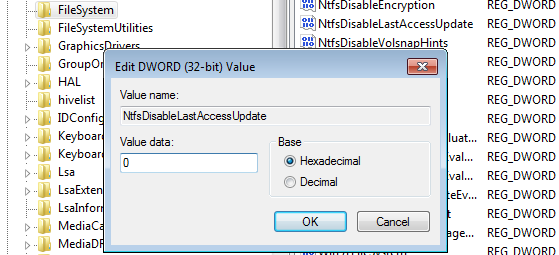
\includegraphics[scale=0.25]{images/lastAccess.png}
                \item Performance reasons
                \item Good for file server
            \end{itemize}
            \item Still updated some times
            \begin{itemize}
                \item File new created
                \item File copied
                \item File moved
            \end{itemize}
        \end{itemize}
    \end{itemize}
\end{frame}


\begin{frame}[fragile]
  \frametitle{5.4 Time Line: Exercise}
  \begin{lstlisting}[basicstyle=\tiny]
Reproduce file system activities
--------------------------------
  
     Thu Jun 27 2013 12:23:08      113 ...b         35-128-1 c:/01.txt
     Thu Jun 27 2013 12:24:20       75 m.cb         37-128-1 c:/02.txt
     Thu Jun 27 2013 12:25:24       75 m.cb         38-128-1 c:/03.txt
                                    75 m...         41-128-1 c:/03-copy.txt
     Thu Jun 27 2013 12:26:05       75 m..b         39-128-1 c:/44.txt
     Thu Jun 27 2013 12:27:00       75 macb         40-128-1 c:/05.txt (deleted)
     Thu Jun 27 2013 12:33:50      113 m.c.         35-128-1 c:/01.txt
     Thu Jun 27 2013 13:07:52       75 .acb         41-128-1 c:/03-copy.txt
     Thu Jun 27 2013 13:10:36       75 ..c.         39-128-1 c:/44.txt
     Thu Jun 27 2013 13:14:20       20 m...         42-128-1 c:/06.txt
     Thu Jun 27 2013 13:56:30       20 .acb         42-128-1 c:/06.txt


File: 01.txt
------------
     Thu Jun 27 2013 12:23:08      113 ...b         35-128-1 c:/01.txt
     Thu Jun 27 2013 12:33:50      113 m.c.         35-128-1 c:/01.txt


File: 02.txt
------------
     Thu Jun 27 2013 12:24:20       75 m.cb         37-128-1 c:/02.txt


-----
  \end{lstlisting}
\end{frame}


\begin{frame}[fragile]
  \frametitle{5.4 Time Line: Exercise}
  \begin{lstlisting}[basicstyle=\tiny]
Reproduce file system activities
--------------------------------
  
     Thu Jun 27 2013 12:23:08      113 ...b         35-128-1 c:/01.txt
     Thu Jun 27 2013 12:24:20       75 m.cb         37-128-1 c:/02.txt
     Thu Jun 27 2013 12:25:24       75 m.cb         38-128-1 c:/03.txt
                                    75 m...         41-128-1 c:/03 - Copy.txt
     Thu Jun 27 2013 12:26:05       75 m..b         39-128-1 c:/44.txt
     Thu Jun 27 2013 12:27:00       75 macb         40-128-1 c:/05.txt (deleted)
     Thu Jun 27 2013 12:33:50      113 m.c.         35-128-1 c:/01.txt
     Thu Jun 27 2013 13:07:52       75 .acb         41-128-1 c:/03 - Copy.txt
     Thu Jun 27 2013 13:10:36       75 ..c.         39-128-1 c:/44.txt
     Thu Jun 27 2013 13:14:20       20 m...         42-128-1 c:/06.txt
     Thu Jun 27 2013 13:56:30       20 .acb         42-128-1 c:/06.txt


File: 03.txt, 03-copy.txt
-------------------------
     Thu Jun 27 2013 12:25:24       75 m.cb         38-128-1 c:/03.txt
				    75 m...         41-128-1 c:/03-copy.txt
     Thu Jun 27 2013 13:07:52       75 .acb         41-128-1 c:/03-copy.txt


File: 02.txt
------------
     Thu Jun 27 2013 12:26:05       75 m..b         39-128-1 c:/44.txt
     Thu Jun 27 2013 13:10:36       75 ..c.         39-128-1 c:/44.txt
-----
  \end{lstlisting}
\end{frame}


\begin{frame}[fragile]
  \frametitle{5.4 Time Line: Exercise}
  \begin{lstlisting}[basicstyle=\tiny]
Reproduce file system activities
--------------------------------
  
     Thu Jun 27 2013 12:23:08      113 ...b         35-128-1 c:/01.txt
     Thu Jun 27 2013 12:24:20       75 m.cb         37-128-1 c:/02.txt
     Thu Jun 27 2013 12:25:24       75 m.cb         38-128-1 c:/03.txt
                                    75 m...         41-128-1 c:/03-copy.txt
     Thu Jun 27 2013 12:26:05       75 m..b         39-128-1 c:/44.txt
     Thu Jun 27 2013 12:27:00       75 macb         40-128-1 c:/05.txt (deleted)
     Thu Jun 27 2013 12:33:50      113 m.c.         35-128-1 c:/01.txt
     Thu Jun 27 2013 13:07:52       75 .acb         41-128-1 c:/03 - Copy.txt
     Thu Jun 27 2013 13:10:36       75 ..c.         39-128-1 c:/44.txt
     Thu Jun 27 2013 13:14:20       20 m...         42-128-1 c:/06.txt
     Thu Jun 27 2013 13:56:30       20 .acb         42-128-1 c:/06.txt


File: 05.txt
------------
     Thu Jun 27 2013 12:27:00       75 macb         40-128-1 c:/05.txt (deleted)


File: 06.txt
------------
     Thu Jun 27 2013 13:14:20       20 m...         42-128-1 c:/06.txt
     Thu Jun 27 2013 13:56:30       20 .acb         42-128-1 c:/06.txt


-----
  \end{lstlisting}
\end{frame}


\begin{frame}[fragile]
  \frametitle{5.4 Time Line: Exercise}
  \begin{lstlisting}[basicstyle=\tiny]
Summary: What could we reproduce                                       Yes/No
-----------------------------------------------------------------------------
  
01.txt
      1. 12:23:08 01.txt -> new create                                 Yes
      6. 12:29:07 01.txt -> modified content                               No
      7. 12:33:50 01.txt -> 2nd modification                           Yes

02.txt
      2. 12:24:20 02.txt -> new create                                 Yes
      8. 12:29:50 02.txt -> open/access file                               No
      9. 12:30:01 02.txt -> close                                          No

03.txt, time-03 - Copy.txt
      3. 12:25:24 03.txt -> new create                                 Yes
     10. 13:07:52 03.txt -> copy to 03-copy.txt                        Yes/No

44.txt
      4. 12:26:05 04.txt -> new create                                 Yes
     11. 13:10:36 04.txt -> rename to 44.txt                           Yes/No

05.txt
      5. 12:27:00 05.txt -> new create                                 Yes
     14. 13:58:07 05.txt -> delete file                                    No

06.txt
     12. 13:14:20 06.txt -> new created on other drive                 Yes/No
     13. 13:56:30 06.txt -> copy to local drive                        Yes
  \end{lstlisting}
\end{frame}


\begin{frame}[fragile]
\frametitle{5.5 Create a Time Line}
  \begin{lstlisting}[basicstyle=\tiny]
$ mkdir time


$ fls -o 2048 -r -m d:/ circl-dfir.dd > time/d.body

          -r    Recursive
          -m    Time machine format
	  D:/   Add D:/ as mountpoint in report


$ cd time
$ mactime -b d.body > d.time
$ less d.time

.....
Wed May 03 2023 16:39:48 134217728 m.c.    113-128-2 d:/NTFS/Challenge_UnDel/ntfs.back
                               48 ...b     114-144-2 d:/Paula (deleted)
                             1246 macb     115-128-2 d:/Paula/Paula.txt (deleted)
                              240 .a.b     116-144-2 d:/RO
                         269483520 .a.b    117-128-2 d:/RO/ro.raw
Wed May 03 2023 16:39:50      240 m.c.     116-144-2 d:/RO
                         269483520 m.c.    117-128-2 d:/RO/ro.raw
                         269483520 .a.b    118-128-2 d:/RO/ro.back
Wed May 03 2023 16:39:51 269483520 m.c.    118-128-2 d:/RO/ro.back
                              144 macb     119-144-2 d:/timeline
                             5936 macb     120-128-2 d:/timeline/c.txt
Wed May 03 2023 16:40:25       48 mac.     114-144-2 d:/Paula (deleted)
  \end{lstlisting}
\end{frame}


\begin{frame}[fragile]
\frametitle{5.5 Create a Time Line}
  \begin{lstlisting}[basicstyle=\tiny]
Limit the timeline to the term Paula
------------------------------------

1.   grep -i paula d.body | grep -v FILE_NAME > paula.body

2.   mactime -b paula.body > paula.time

3.   less paula.time


     Wed May 03 2023 16:39:48       48 ...b     114-144-2 d:/Paula (deleted)
                                  1246 macb     115-128-2 d:/Paula/Paula.txt (deleted)
     Wed May 03 2023 16:40:25       48 mac.     114-144-2 d:/Paula (deleted)



Can you tell the storry?
------------------------








_
  \end{lstlisting}
\end{frame}


\begin{frame}[fragile]
\frametitle{5.5 Create a Time Line}
  \begin{lstlisting}[basicstyle=\tiny]
Limit the timeline to the term Paula
------------------------------------

1.   grep -i paula d.body | grep -v FILE_NAME > paula.body

2.   mactime -b paula.body > paula.time

3.   less paula.time


     Wed May 03 2023 16:39:48       48 ...b     114-144-2 d:/Paula (deleted)
                                  1246 macb     115-128-2 d:/Paula/Paula.txt (deleted)
     Wed May 03 2023 16:40:25       48 mac.     114-144-2 d:/Paula (deleted)



Can you tell the storry?
------------------------

1. Wed May 03 2023 16:39:48	Directory 'Paula' created in the root directory

2. Wed May 03 2023 16:39:48	File 'Paula.txt' created in directory 'Paula'

3.				Directory 'Paula' and file 'Paula.txt' got deleted

4. Wed May 03 2023 16:40:25	Directory 'Paula' last access, content/meta modified
				-> Most likely due to file 'Paula.txt deleted
  \end{lstlisting}
\end{frame}


\begin{frame}[fragile]
\frametitle{5.6 Challenge: Time Line Analysis}
  \begin{lstlisting}[basicstyle=\tiny]
2009 M57-Jean
-------------

https://digitalcorpora.org/corpora/scenarios/m57-jean/

	M57-Jean/
	|-- original_disk
	|   |-- nps-2008-jean.E01
	|   |-- nps-2008-jean.E02
	|-- slides
	    |-- M57-Jean.pdf
	    |-- M57-Jean_Solution.pdf

	2 directories, 4 files


$ ewfinfo original_disk/nps-2008-jean.E01
$ ewfexport original_disk/nps-2008-jean.E01


$ mmls ../nps-2008-jean.raw.raw
$ fls -r -o 63 -m C: ../nps-2008-jean.raw.raw > c.body
$ mactime -z UTC -b c.body > c.time
$ less c.time


--> Search for the file m57biz.xls
  \end{lstlisting}
\end{frame}





\include{f26_car}
\include{f27_str}
\include{f28_cha}
%
% This work is licensed under a Creative Commons Attribution-ShareAlike 4.0 International License.
% http://creativecommons.org/licenses/by-sa/4.0/
%

% DO NOT COMPILE THIS FILE DIRECTLY!
% This is included by the other .tex files.


\begin{frame}
    \includegraphics[scale=0.3]{images/logo-circl-Forensics.png}
    \begin{itemize}
        \item[]
        \item[]
        \item[] 9. Bibliography and Outlook
    \end{itemize}
\end{frame}


\begin{frame}[fragile]
  \frametitle{9. Bibliography}
  \begin{itemize}
      \item Digital Forensics with Kali Linux
        \begin{itemize}
            \item[] Shiva V.N. Parasram
            \item[] Packt Publishing
            \item[] ISBN-13: 978-1-78862-500-5
        \end{itemize}
      \item[]
      \item Practical Forensic Imaging
        \begin{itemize}
            \item[] Bruce Nikkel
            \item[] No Starch Press
            \item[] ISBN-13: 978-1-59-327793-2
        \end{itemize}
      \item[]
      \item Digital Forensics with Open Source Tools
        \begin{itemize}
            \item[] Cory Altheide, Harlan Carvey
            \item[] Syngress
            \item[] ISBN-13: 978-1-59-749586-8
        \end{itemize}
  \end{itemize}
\end{frame}


\begin{frame}
  \frametitle{9. Bibliography}
  \begin{itemize}
      \item File System Forensic Analysis
        \begin{itemize}
            \item[] Brian Carrier
            \item[] Pearson Education
            \item[] ISBN-13: 978-0-32-126817-4
        \end{itemize}
      \item[]
      \item Forensic Computing: A Practitioner’s Guide
        \begin{itemize}
            \item[] Anthony Sammes, Brian Jenkinson
            \item[] Springer
            \item[] ISBN-13: 978-1-85-233299-0
        \end{itemize}
      \item[]
      \item[] 
        \begin{itemize}
            \item[]
            \item[]
            \item[] 
        \end{itemize}
  \end{itemize}
\end{frame}


\begin{frame}
  \frametitle{9. Outlook}
  \begin{itemize}
      \item[] CIRCL DFIR 1.0.2
      \begin{itemize}
          \item[]
          \item[] EXT File System
          \item[]
      \end{itemize}
  \end{itemize}
\end{frame}





\begin{frame}
  \frametitle{Overview}
  \begin{itemize}
  \item[]
      \begin{enumerate}
          \item File System Analysis - Overview
          \item FAT - File Allocation Table
          \item NTFS - New Technology File System
          \item NTFS - Advanced
          \item File System Time Line
          \item 
          \item Carving and String Search
          \item Forensics Challenges
          \item Bibliography and Outlook
      \end{enumerate}
  \end{itemize}
\end{frame}

\end{document}

